% Created by tikzDevice version 0.7.0 on 2014-07-29 12:26:41
% !TEX encoding = UTF-8 Unicode
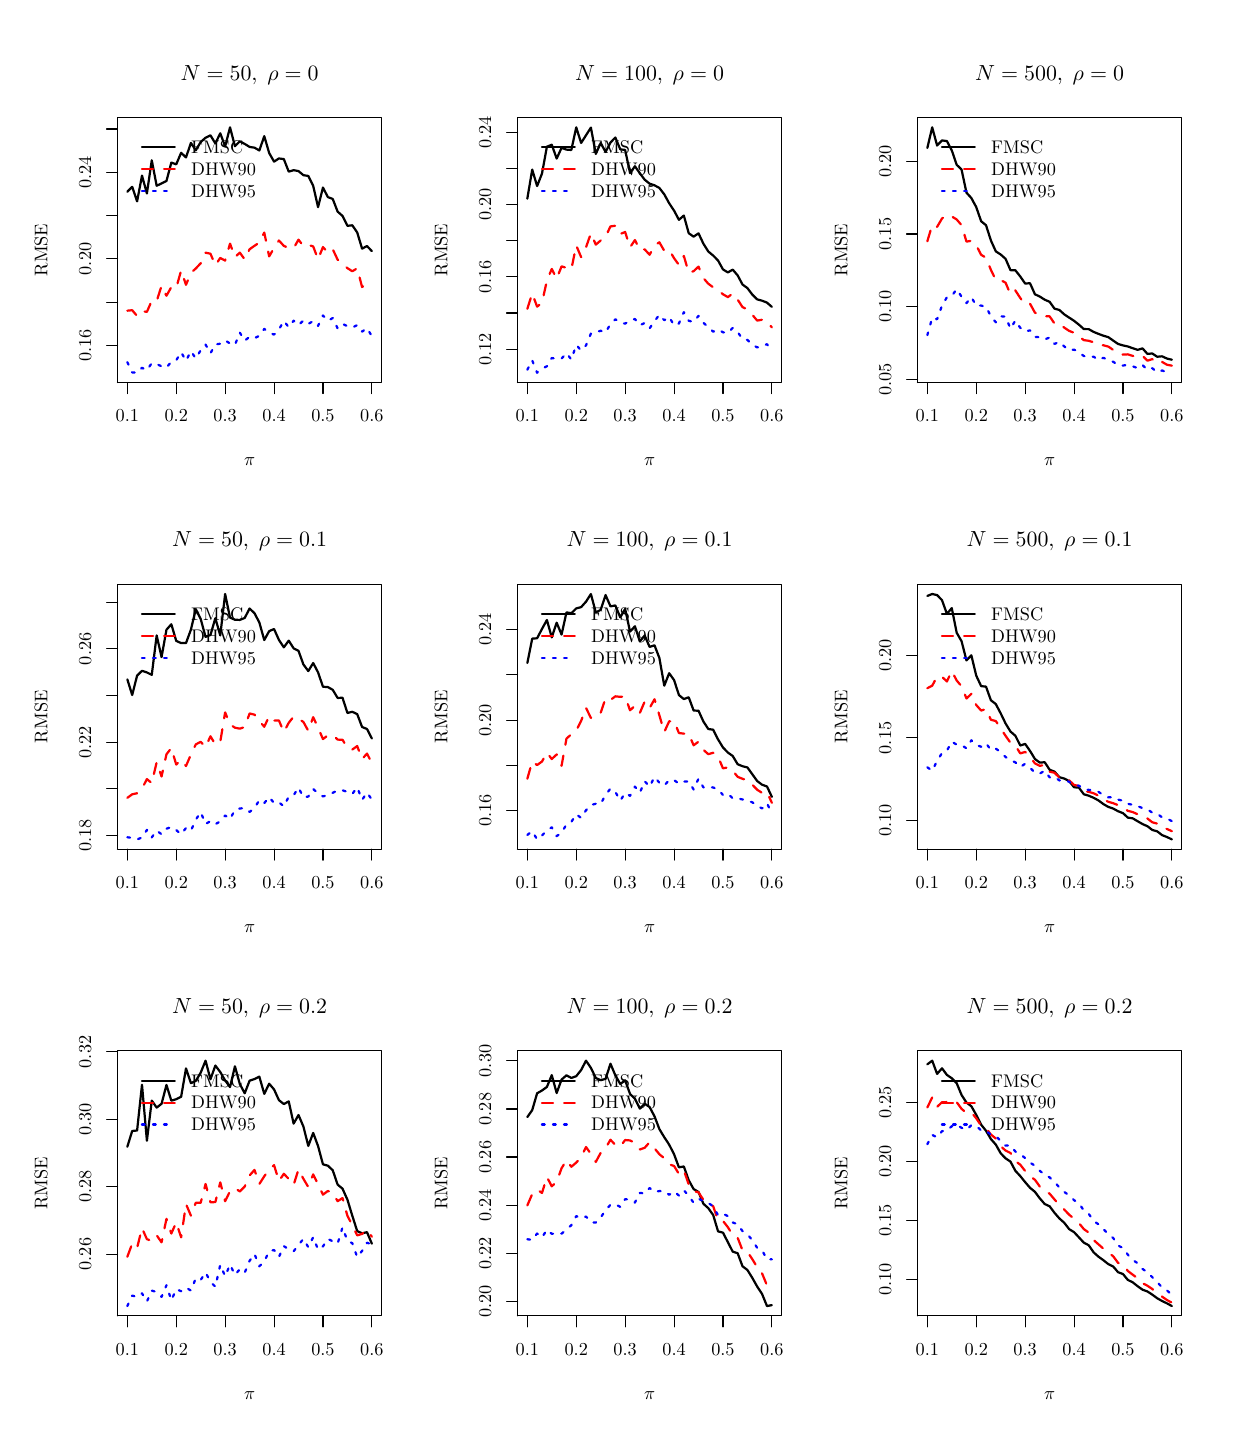
\begin{tikzpicture}[x=1pt,y=1pt]
\definecolor[named]{fillColor}{rgb}{1.00,1.00,1.00}
\path[use as bounding box,fill=fillColor,fill opacity=0.00] (0,0) rectangle (433.62,505.89);
\begin{scope}
\path[clip] ( 32.47,377.65) rectangle (127.91,473.42);
\definecolor[named]{drawColor}{rgb}{0.00,0.00,0.00}

\path[draw=drawColor,line width= 0.8pt,line join=round,line cap=round] ( 36.01,446.60) --
	( 37.77,448.37) --
	( 39.54,443.11) --
	( 41.31,452.44) --
	( 43.08,445.98) --
	( 44.84,457.95) --
	( 46.61,448.76) --
	( 48.38,449.60) --
	( 50.15,450.49) --
	( 51.91,457.13) --
	( 53.68,456.50) --
	( 55.45,460.67) --
	( 57.21,459.00) --
	( 58.98,464.24) --
	( 60.75,461.56) --
	( 62.52,464.58) --
	( 64.28,466.11) --
	( 66.05,466.99) --
	( 67.82,464.05) --
	( 69.59,467.72) --
	( 71.35,462.97) --
	( 73.12,469.87) --
	( 74.89,463.06) --
	( 76.66,464.84) --
	( 78.42,463.88) --
	( 80.19,462.79) --
	( 81.96,462.52) --
	( 83.72,461.51) --
	( 85.49,466.69) --
	( 87.26,460.60) --
	( 89.03,457.48) --
	( 90.79,458.63) --
	( 92.56,458.39) --
	( 94.33,453.87) --
	( 96.10,454.38) --
	( 97.86,454.07) --
	( 99.63,452.58) --
	(101.40,452.31) --
	(103.17,448.74) --
	(104.93,441.02) --
	(106.70,448.12) --
	(108.47,444.66) --
	(110.23,444.00) --
	(112.00,439.42) --
	(113.77,437.85) --
	(115.54,434.28) --
	(117.30,434.48) --
	(119.07,431.90) --
	(120.84,426.03) --
	(122.61,426.98) --
	(124.37,425.14);
\end{scope}
\begin{scope}
\path[clip] (  0.00,  0.00) rectangle (433.62,505.89);
\definecolor[named]{drawColor}{rgb}{0.00,0.00,0.00}

\path[draw=drawColor,line width= 0.4pt,line join=round,line cap=round] ( 36.01,377.65) -- (124.37,377.65);

\path[draw=drawColor,line width= 0.4pt,line join=round,line cap=round] ( 36.01,377.65) -- ( 36.01,373.69);

\path[draw=drawColor,line width= 0.4pt,line join=round,line cap=round] ( 53.68,377.65) -- ( 53.68,373.69);

\path[draw=drawColor,line width= 0.4pt,line join=round,line cap=round] ( 71.35,377.65) -- ( 71.35,373.69);

\path[draw=drawColor,line width= 0.4pt,line join=round,line cap=round] ( 89.03,377.65) -- ( 89.03,373.69);

\path[draw=drawColor,line width= 0.4pt,line join=round,line cap=round] (106.70,377.65) -- (106.70,373.69);

\path[draw=drawColor,line width= 0.4pt,line join=round,line cap=round] (124.37,377.65) -- (124.37,373.69);

\node[text=drawColor,anchor=base,inner sep=0pt, outer sep=0pt, scale=  0.66] at ( 36.01,363.40) {0.1};

\node[text=drawColor,anchor=base,inner sep=0pt, outer sep=0pt, scale=  0.66] at ( 53.68,363.40) {0.2};

\node[text=drawColor,anchor=base,inner sep=0pt, outer sep=0pt, scale=  0.66] at ( 71.35,363.40) {0.3};

\node[text=drawColor,anchor=base,inner sep=0pt, outer sep=0pt, scale=  0.66] at ( 89.03,363.40) {0.4};

\node[text=drawColor,anchor=base,inner sep=0pt, outer sep=0pt, scale=  0.66] at (106.70,363.40) {0.5};

\node[text=drawColor,anchor=base,inner sep=0pt, outer sep=0pt, scale=  0.66] at (124.37,363.40) {0.6};

\path[draw=drawColor,line width= 0.4pt,line join=round,line cap=round] ( 32.47,391.03) -- ( 32.47,469.27);

\path[draw=drawColor,line width= 0.4pt,line join=round,line cap=round] ( 32.47,391.03) -- ( 28.51,391.03);

\path[draw=drawColor,line width= 0.4pt,line join=round,line cap=round] ( 32.47,406.67) -- ( 28.51,406.67);

\path[draw=drawColor,line width= 0.4pt,line join=round,line cap=round] ( 32.47,422.32) -- ( 28.51,422.32);

\path[draw=drawColor,line width= 0.4pt,line join=round,line cap=round] ( 32.47,437.97) -- ( 28.51,437.97);

\path[draw=drawColor,line width= 0.4pt,line join=round,line cap=round] ( 32.47,453.62) -- ( 28.51,453.62);

\path[draw=drawColor,line width= 0.4pt,line join=round,line cap=round] ( 32.47,469.27) -- ( 28.51,469.27);

\node[text=drawColor,rotate= 90.00,anchor=base,inner sep=0pt, outer sep=0pt, scale=  0.66] at ( 22.97,391.03) {0.16};

\node[text=drawColor,rotate= 90.00,anchor=base,inner sep=0pt, outer sep=0pt, scale=  0.66] at ( 22.97,422.32) {0.20};

\node[text=drawColor,rotate= 90.00,anchor=base,inner sep=0pt, outer sep=0pt, scale=  0.66] at ( 22.97,453.62) {0.24};

\path[draw=drawColor,line width= 0.4pt,line join=round,line cap=round] ( 32.47,377.65) --
	(127.91,377.65) --
	(127.91,473.42) --
	( 32.47,473.42) --
	( 32.47,377.65);
\end{scope}
\begin{scope}
\path[clip] (  0.00,337.26) rectangle (144.54,505.89);
\definecolor[named]{drawColor}{rgb}{0.00,0.00,0.00}

\node[text=drawColor,anchor=base,inner sep=0pt, outer sep=0pt, scale=  0.79] at ( 80.19,486.92) {\bfseries $N=50, \;\rho=0$};

\node[text=drawColor,anchor=base,inner sep=0pt, outer sep=0pt, scale=  0.66] at ( 80.19,347.56) {$\pi$};

\node[text=drawColor,rotate= 90.00,anchor=base,inner sep=0pt, outer sep=0pt, scale=  0.66] at (  7.13,425.53) {RMSE};
\end{scope}
\begin{scope}
\path[clip] ( 32.47,377.65) rectangle (127.91,473.42);
\definecolor[named]{drawColor}{rgb}{1.00,0.00,0.00}

\path[draw=drawColor,line width= 0.8pt,dash pattern=on 4pt off 4pt ,line join=round,line cap=round] ( 36.01,403.62) --
	( 37.77,403.79) --
	( 39.54,401.70) --
	( 41.31,403.48) --
	( 43.08,403.18) --
	( 44.84,407.21) --
	( 46.61,407.06) --
	( 48.38,412.62) --
	( 50.15,409.02) --
	( 51.91,412.16) --
	( 53.68,411.83) --
	( 55.45,418.14) --
	( 57.21,412.97) --
	( 58.98,417.27) --
	( 60.75,418.87) --
	( 62.52,420.76) --
	( 64.28,424.58) --
	( 66.05,424.20) --
	( 67.82,420.04) --
	( 69.59,422.67) --
	( 71.35,421.72) --
	( 73.12,427.85) --
	( 74.89,422.96) --
	( 76.66,424.60) --
	( 78.42,422.14) --
	( 80.19,425.82) --
	( 81.96,427.07) --
	( 83.72,428.24) --
	( 85.49,431.85) --
	( 87.26,423.24) --
	( 89.03,426.27) --
	( 90.79,428.98) --
	( 92.56,427.04) --
	( 94.33,426.28) --
	( 96.10,426.21) --
	( 97.86,429.28) --
	( 99.63,426.96) --
	(101.40,427.39) --
	(103.17,426.84) --
	(104.93,422.17) --
	(106.70,426.62) --
	(108.47,424.62) --
	(110.23,425.83) --
	(112.00,422.06) --
	(113.77,420.43) --
	(115.54,418.99) --
	(117.30,417.86) --
	(119.07,418.92) --
	(120.84,412.17) --
	(122.61,413.41) --
	(124.37,412.39);
\definecolor[named]{drawColor}{rgb}{0.00,0.00,1.00}

\path[draw=drawColor,line width= 0.8pt,dash pattern=on 1pt off 3pt ,line join=round,line cap=round] ( 36.01,385.02) --
	( 37.77,381.32) --
	( 39.54,381.20) --
	( 41.31,382.99) --
	( 43.08,382.07) --
	( 44.84,384.67) --
	( 46.61,384.31) --
	( 48.38,383.53) --
	( 50.15,383.03) --
	( 51.91,385.18) --
	( 53.68,385.70) --
	( 55.45,388.63) --
	( 57.21,385.49) --
	( 58.98,389.02) --
	( 60.75,386.35) --
	( 62.52,389.35) --
	( 64.28,391.36) --
	( 66.05,388.23) --
	( 67.82,391.43) --
	( 69.59,391.68) --
	( 71.35,392.90) --
	( 73.12,391.76) --
	( 74.89,391.23) --
	( 76.66,395.69) --
	( 78.42,392.78) --
	( 80.19,394.18) --
	( 81.96,393.69) --
	( 83.72,394.56) --
	( 85.49,397.03) --
	( 87.26,395.59) --
	( 89.03,394.99) --
	( 90.79,396.82) --
	( 92.56,399.94) --
	( 94.33,397.65) --
	( 96.10,400.00) --
	( 97.86,398.38) --
	( 99.63,400.10) --
	(101.40,398.84) --
	(103.17,399.86) --
	(104.93,398.13) --
	(106.70,401.89) --
	(108.47,399.97) --
	(110.23,400.95) --
	(112.00,397.23) --
	(113.77,398.87) --
	(115.54,398.00) --
	(117.30,397.54) --
	(119.07,398.40) --
	(120.84,396.03) --
	(122.61,397.35) --
	(124.37,394.40);
\definecolor[named]{drawColor}{rgb}{0.00,0.00,0.00}

\path[draw=drawColor,line width= 0.8pt,line join=round,line cap=round] ( 41.28,462.63) -- ( 53.16,462.63);
\definecolor[named]{drawColor}{rgb}{1.00,0.00,0.00}

\path[draw=drawColor,line width= 0.8pt,dash pattern=on 4pt off 4pt ,line join=round,line cap=round] ( 41.28,454.71) -- ( 53.16,454.71);
\definecolor[named]{drawColor}{rgb}{0.00,0.00,1.00}

\path[draw=drawColor,line width= 0.8pt,dash pattern=on 1pt off 3pt ,line join=round,line cap=round] ( 41.28,446.79) -- ( 53.16,446.79);
\definecolor[named]{drawColor}{rgb}{0.00,0.00,0.00}

\node[text=drawColor,anchor=base west,inner sep=0pt, outer sep=0pt, scale=  0.66] at ( 59.10,460.35) {FMSC};

\node[text=drawColor,anchor=base west,inner sep=0pt, outer sep=0pt, scale=  0.66] at ( 59.10,452.43) {DHW90};

\node[text=drawColor,anchor=base west,inner sep=0pt, outer sep=0pt, scale=  0.66] at ( 59.10,444.51) {DHW95};
\end{scope}
\begin{scope}
\path[clip] (177.01,377.65) rectangle (272.45,473.42);
\definecolor[named]{drawColor}{rgb}{0.00,0.00,0.00}

\path[draw=drawColor,line width= 0.8pt,line join=round,line cap=round] (180.55,444.09) --
	(182.31,454.61) --
	(184.08,448.65) --
	(185.85,453.18) --
	(187.62,462.87) --
	(189.38,463.58) --
	(191.15,458.59) --
	(192.92,462.46) --
	(194.69,461.82) --
	(196.45,461.69) --
	(198.22,469.87) --
	(199.99,464.22) --
	(201.75,467.00) --
	(203.52,469.78) --
	(205.29,460.27) --
	(207.06,464.21) --
	(208.82,460.96) --
	(210.59,464.38) --
	(212.36,466.20) --
	(214.13,461.91) --
	(215.89,461.71) --
	(217.66,453.36) --
	(219.43,455.79) --
	(221.20,453.29) --
	(222.96,450.95) --
	(224.73,449.51) --
	(226.50,448.92) --
	(228.26,447.97) --
	(230.03,445.66) --
	(231.80,442.44) --
	(233.57,439.78) --
	(235.33,436.45) --
	(237.10,438.00) --
	(238.87,431.61) --
	(240.64,430.37) --
	(242.40,431.57) --
	(244.17,427.83) --
	(245.94,425.00) --
	(247.71,423.53) --
	(249.47,421.74) --
	(251.24,418.54) --
	(253.01,417.44) --
	(254.77,418.46) --
	(256.54,416.38) --
	(258.31,413.07) --
	(260.08,411.78) --
	(261.84,409.44) --
	(263.61,407.70) --
	(265.38,407.23) --
	(267.15,406.53) --
	(268.91,404.98);
\end{scope}
\begin{scope}
\path[clip] (  0.00,  0.00) rectangle (433.62,505.89);
\definecolor[named]{drawColor}{rgb}{0.00,0.00,0.00}

\path[draw=drawColor,line width= 0.4pt,line join=round,line cap=round] (180.55,377.65) -- (268.91,377.65);

\path[draw=drawColor,line width= 0.4pt,line join=round,line cap=round] (180.55,377.65) -- (180.55,373.69);

\path[draw=drawColor,line width= 0.4pt,line join=round,line cap=round] (198.22,377.65) -- (198.22,373.69);

\path[draw=drawColor,line width= 0.4pt,line join=round,line cap=round] (215.89,377.65) -- (215.89,373.69);

\path[draw=drawColor,line width= 0.4pt,line join=round,line cap=round] (233.57,377.65) -- (233.57,373.69);

\path[draw=drawColor,line width= 0.4pt,line join=round,line cap=round] (251.24,377.65) -- (251.24,373.69);

\path[draw=drawColor,line width= 0.4pt,line join=round,line cap=round] (268.91,377.65) -- (268.91,373.69);

\node[text=drawColor,anchor=base,inner sep=0pt, outer sep=0pt, scale=  0.66] at (180.55,363.40) {0.1};

\node[text=drawColor,anchor=base,inner sep=0pt, outer sep=0pt, scale=  0.66] at (198.22,363.40) {0.2};

\node[text=drawColor,anchor=base,inner sep=0pt, outer sep=0pt, scale=  0.66] at (215.89,363.40) {0.3};

\node[text=drawColor,anchor=base,inner sep=0pt, outer sep=0pt, scale=  0.66] at (233.57,363.40) {0.4};

\node[text=drawColor,anchor=base,inner sep=0pt, outer sep=0pt, scale=  0.66] at (251.24,363.40) {0.5};

\node[text=drawColor,anchor=base,inner sep=0pt, outer sep=0pt, scale=  0.66] at (268.91,363.40) {0.6};

\path[draw=drawColor,line width= 0.4pt,line join=round,line cap=round] (177.01,389.70) -- (177.01,468.14);

\path[draw=drawColor,line width= 0.4pt,line join=round,line cap=round] (177.01,389.70) -- (173.05,389.70);

\path[draw=drawColor,line width= 0.4pt,line join=round,line cap=round] (177.01,402.77) -- (173.05,402.77);

\path[draw=drawColor,line width= 0.4pt,line join=round,line cap=round] (177.01,415.84) -- (173.05,415.84);

\path[draw=drawColor,line width= 0.4pt,line join=round,line cap=round] (177.01,428.92) -- (173.05,428.92);

\path[draw=drawColor,line width= 0.4pt,line join=round,line cap=round] (177.01,441.99) -- (173.05,441.99);

\path[draw=drawColor,line width= 0.4pt,line join=round,line cap=round] (177.01,455.07) -- (173.05,455.07);

\path[draw=drawColor,line width= 0.4pt,line join=round,line cap=round] (177.01,468.14) -- (173.05,468.14);

\node[text=drawColor,rotate= 90.00,anchor=base,inner sep=0pt, outer sep=0pt, scale=  0.66] at (167.51,389.70) {0.12};

\node[text=drawColor,rotate= 90.00,anchor=base,inner sep=0pt, outer sep=0pt, scale=  0.66] at (167.51,415.84) {0.16};

\node[text=drawColor,rotate= 90.00,anchor=base,inner sep=0pt, outer sep=0pt, scale=  0.66] at (167.51,441.99) {0.20};

\node[text=drawColor,rotate= 90.00,anchor=base,inner sep=0pt, outer sep=0pt, scale=  0.66] at (167.51,468.14) {0.24};

\path[draw=drawColor,line width= 0.4pt,line join=round,line cap=round] (177.01,377.65) --
	(272.45,377.65) --
	(272.45,473.42) --
	(177.01,473.42) --
	(177.01,377.65);
\end{scope}
\begin{scope}
\path[clip] (144.54,337.26) rectangle (289.08,505.89);
\definecolor[named]{drawColor}{rgb}{0.00,0.00,0.00}

\node[text=drawColor,anchor=base,inner sep=0pt, outer sep=0pt, scale=  0.79] at (224.73,486.92) {\bfseries $N=100, \;\rho=0$};

\node[text=drawColor,anchor=base,inner sep=0pt, outer sep=0pt, scale=  0.66] at (224.73,347.56) {$\pi$};

\node[text=drawColor,rotate= 90.00,anchor=base,inner sep=0pt, outer sep=0pt, scale=  0.66] at (151.67,425.53) {RMSE};
\end{scope}
\begin{scope}
\path[clip] (177.01,377.65) rectangle (272.45,473.42);
\definecolor[named]{drawColor}{rgb}{1.00,0.00,0.00}

\path[draw=drawColor,line width= 0.8pt,dash pattern=on 4pt off 4pt ,line join=round,line cap=round] (180.55,404.29) --
	(182.31,409.86) --
	(184.08,405.07) --
	(185.85,406.48) --
	(187.62,414.50) --
	(189.38,418.70) --
	(191.15,415.16) --
	(192.92,419.65) --
	(194.69,419.08) --
	(196.45,418.57) --
	(198.22,427.20) --
	(199.99,422.97) --
	(201.75,426.52) --
	(203.52,431.59) --
	(205.29,427.48) --
	(207.06,428.99) --
	(208.82,430.36) --
	(210.59,434.07) --
	(212.36,434.31) --
	(214.13,431.34) --
	(215.89,432.05) --
	(217.66,426.52) --
	(219.43,429.15) --
	(221.20,425.54) --
	(222.96,425.76) --
	(224.73,423.82) --
	(226.50,427.18) --
	(228.26,428.34) --
	(230.03,425.25) --
	(231.80,425.55) --
	(233.57,422.60) --
	(235.33,420.14) --
	(237.10,423.41) --
	(238.87,417.34) --
	(240.64,417.90) --
	(242.40,419.55) --
	(244.17,415.40) --
	(245.94,413.36) --
	(247.71,412.06) --
	(249.47,411.01) --
	(251.24,409.56) --
	(253.01,408.52) --
	(254.77,409.83) --
	(256.54,407.64) --
	(258.31,404.90) --
	(260.08,404.07) --
	(261.84,402.13) --
	(263.61,400.04) --
	(265.38,400.35) --
	(267.15,399.73) --
	(268.91,397.58);
\definecolor[named]{drawColor}{rgb}{0.00,0.00,1.00}

\path[draw=drawColor,line width= 0.8pt,dash pattern=on 1pt off 3pt ,line join=round,line cap=round] (180.55,382.28) --
	(182.31,385.66) --
	(184.08,381.20) --
	(185.85,382.64) --
	(187.62,383.54) --
	(189.38,386.52) --
	(191.15,386.23) --
	(192.92,386.31) --
	(194.69,388.30) --
	(196.45,385.94) --
	(198.22,391.26) --
	(199.99,389.23) --
	(201.75,391.08) --
	(203.52,395.35) --
	(205.29,395.86) --
	(207.06,396.36) --
	(208.82,395.74) --
	(210.59,398.79) --
	(212.36,400.50) --
	(214.13,399.33) --
	(215.89,398.94) --
	(217.66,400.08) --
	(219.43,400.61) --
	(221.20,398.33) --
	(222.96,399.19) --
	(224.73,397.24) --
	(226.50,399.83) --
	(228.26,402.14) --
	(230.03,400.18) --
	(231.80,401.40) --
	(233.57,398.29) --
	(235.33,399.01) --
	(237.10,403.08) --
	(238.87,399.98) --
	(240.64,399.55) --
	(242.40,401.73) --
	(244.17,399.25) --
	(245.94,397.65) --
	(247.71,396.04) --
	(249.47,396.83) --
	(251.24,395.82) --
	(253.01,395.53) --
	(254.77,397.42) --
	(256.54,395.92) --
	(258.31,393.37) --
	(260.08,393.05) --
	(261.84,391.28) --
	(263.61,390.36) --
	(265.38,390.64) --
	(267.15,391.53) --
	(268.91,389.15);
\definecolor[named]{drawColor}{rgb}{0.00,0.00,0.00}

\path[draw=drawColor,line width= 0.8pt,line join=round,line cap=round] (185.82,462.63) -- (197.70,462.63);
\definecolor[named]{drawColor}{rgb}{1.00,0.00,0.00}

\path[draw=drawColor,line width= 0.8pt,dash pattern=on 4pt off 4pt ,line join=round,line cap=round] (185.82,454.71) -- (197.70,454.71);
\definecolor[named]{drawColor}{rgb}{0.00,0.00,1.00}

\path[draw=drawColor,line width= 0.8pt,dash pattern=on 1pt off 3pt ,line join=round,line cap=round] (185.82,446.79) -- (197.70,446.79);
\definecolor[named]{drawColor}{rgb}{0.00,0.00,0.00}

\node[text=drawColor,anchor=base west,inner sep=0pt, outer sep=0pt, scale=  0.66] at (203.64,460.35) {FMSC};

\node[text=drawColor,anchor=base west,inner sep=0pt, outer sep=0pt, scale=  0.66] at (203.64,452.43) {DHW90};

\node[text=drawColor,anchor=base west,inner sep=0pt, outer sep=0pt, scale=  0.66] at (203.64,444.51) {DHW95};
\end{scope}
\begin{scope}
\path[clip] (321.55,377.65) rectangle (416.99,473.42);
\definecolor[named]{drawColor}{rgb}{0.00,0.00,0.00}

\path[draw=drawColor,line width= 0.8pt,line join=round,line cap=round] (325.09,462.41) --
	(326.85,469.87) --
	(328.62,463.30) --
	(330.39,465.14) --
	(332.16,464.90) --
	(333.92,461.55) --
	(335.69,456.35) --
	(337.46,454.60) --
	(339.23,446.26) --
	(340.99,444.32) --
	(342.76,441.05) --
	(344.53,435.94) --
	(346.29,434.51) --
	(348.06,428.99) --
	(349.83,425.06) --
	(351.60,423.91) --
	(353.36,422.35) --
	(355.13,418.27) --
	(356.90,418.21) --
	(358.67,415.97) --
	(360.43,413.44) --
	(362.20,413.53) --
	(363.97,409.55) --
	(365.74,408.71) --
	(367.50,407.59) --
	(369.27,406.84) --
	(371.04,404.35) --
	(372.80,403.88) --
	(374.57,402.29) --
	(376.34,401.11) --
	(378.11,399.96) --
	(379.87,398.56) --
	(381.64,396.97) --
	(383.41,396.95) --
	(385.18,395.95) --
	(386.94,395.24) --
	(388.71,394.57) --
	(390.48,394.06) --
	(392.25,392.81) --
	(394.01,391.60) --
	(395.78,391.07) --
	(397.55,390.69) --
	(399.31,390.05) --
	(401.08,389.47) --
	(402.85,390.00) --
	(404.62,388.00) --
	(406.38,388.16) --
	(408.15,386.98) --
	(409.92,387.13) --
	(411.69,386.31) --
	(413.45,385.90);
\end{scope}
\begin{scope}
\path[clip] (  0.00,  0.00) rectangle (433.62,505.89);
\definecolor[named]{drawColor}{rgb}{0.00,0.00,0.00}

\path[draw=drawColor,line width= 0.4pt,line join=round,line cap=round] (325.09,377.65) -- (413.45,377.65);

\path[draw=drawColor,line width= 0.4pt,line join=round,line cap=round] (325.09,377.65) -- (325.09,373.69);

\path[draw=drawColor,line width= 0.4pt,line join=round,line cap=round] (342.76,377.65) -- (342.76,373.69);

\path[draw=drawColor,line width= 0.4pt,line join=round,line cap=round] (360.43,377.65) -- (360.43,373.69);

\path[draw=drawColor,line width= 0.4pt,line join=round,line cap=round] (378.11,377.65) -- (378.11,373.69);

\path[draw=drawColor,line width= 0.4pt,line join=round,line cap=round] (395.78,377.65) -- (395.78,373.69);

\path[draw=drawColor,line width= 0.4pt,line join=round,line cap=round] (413.45,377.65) -- (413.45,373.69);

\node[text=drawColor,anchor=base,inner sep=0pt, outer sep=0pt, scale=  0.66] at (325.09,363.40) {0.1};

\node[text=drawColor,anchor=base,inner sep=0pt, outer sep=0pt, scale=  0.66] at (342.76,363.40) {0.2};

\node[text=drawColor,anchor=base,inner sep=0pt, outer sep=0pt, scale=  0.66] at (360.43,363.40) {0.3};

\node[text=drawColor,anchor=base,inner sep=0pt, outer sep=0pt, scale=  0.66] at (378.11,363.40) {0.4};

\node[text=drawColor,anchor=base,inner sep=0pt, outer sep=0pt, scale=  0.66] at (395.78,363.40) {0.5};

\node[text=drawColor,anchor=base,inner sep=0pt, outer sep=0pt, scale=  0.66] at (413.45,363.40) {0.6};

\path[draw=drawColor,line width= 0.4pt,line join=round,line cap=round] (321.55,378.88) -- (321.55,457.55);

\path[draw=drawColor,line width= 0.4pt,line join=round,line cap=round] (321.55,378.88) -- (317.59,378.88);

\path[draw=drawColor,line width= 0.4pt,line join=round,line cap=round] (321.55,405.10) -- (317.59,405.10);

\path[draw=drawColor,line width= 0.4pt,line join=round,line cap=round] (321.55,431.33) -- (317.59,431.33);

\path[draw=drawColor,line width= 0.4pt,line join=round,line cap=round] (321.55,457.55) -- (317.59,457.55);

\node[text=drawColor,rotate= 90.00,anchor=base,inner sep=0pt, outer sep=0pt, scale=  0.66] at (312.05,378.88) {0.05};

\node[text=drawColor,rotate= 90.00,anchor=base,inner sep=0pt, outer sep=0pt, scale=  0.66] at (312.05,405.10) {0.10};

\node[text=drawColor,rotate= 90.00,anchor=base,inner sep=0pt, outer sep=0pt, scale=  0.66] at (312.05,431.33) {0.15};

\node[text=drawColor,rotate= 90.00,anchor=base,inner sep=0pt, outer sep=0pt, scale=  0.66] at (312.05,457.55) {0.20};

\path[draw=drawColor,line width= 0.4pt,line join=round,line cap=round] (321.55,377.65) --
	(416.99,377.65) --
	(416.99,473.42) --
	(321.55,473.42) --
	(321.55,377.65);
\end{scope}
\begin{scope}
\path[clip] (289.08,337.26) rectangle (433.62,505.89);
\definecolor[named]{drawColor}{rgb}{0.00,0.00,0.00}

\node[text=drawColor,anchor=base,inner sep=0pt, outer sep=0pt, scale=  0.79] at (369.27,486.92) {\bfseries $N=500, \;\rho=0$};

\node[text=drawColor,anchor=base,inner sep=0pt, outer sep=0pt, scale=  0.66] at (369.27,347.56) {$\pi$};

\node[text=drawColor,rotate= 90.00,anchor=base,inner sep=0pt, outer sep=0pt, scale=  0.66] at (296.21,425.53) {RMSE};
\end{scope}
\begin{scope}
\path[clip] (321.55,377.65) rectangle (416.99,473.42);
\definecolor[named]{drawColor}{rgb}{1.00,0.00,0.00}

\path[draw=drawColor,line width= 0.8pt,dash pattern=on 4pt off 4pt ,line join=round,line cap=round] (325.09,428.70) --
	(326.85,434.61) --
	(328.62,433.90) --
	(330.39,436.92) --
	(332.16,438.19) --
	(333.92,437.67) --
	(335.69,436.58) --
	(337.46,434.52) --
	(339.23,428.58) --
	(340.99,428.88) --
	(342.76,427.27) --
	(344.53,423.81) --
	(346.29,422.74) --
	(348.06,418.37) --
	(349.83,414.70) --
	(351.60,414.66) --
	(353.36,413.74) --
	(355.13,409.53) --
	(356.90,410.94) --
	(358.67,408.19) --
	(360.43,405.94) --
	(362.20,406.13) --
	(363.97,402.90) --
	(365.74,402.15) --
	(367.50,401.58) --
	(369.27,401.58) --
	(371.04,398.99) --
	(372.80,398.95) --
	(374.57,397.49) --
	(376.34,396.31) --
	(378.11,395.63) --
	(379.87,394.31) --
	(381.64,392.98) --
	(383.41,392.74) --
	(385.18,392.18) --
	(386.94,391.26) --
	(388.71,391.12) --
	(390.48,390.64) --
	(392.25,389.45) --
	(394.01,388.32) --
	(395.78,387.75) --
	(397.55,387.84) --
	(399.31,387.28) --
	(401.08,386.77) --
	(402.85,387.29) --
	(404.62,385.55) --
	(406.38,386.11) --
	(408.15,384.54) --
	(409.92,385.09) --
	(411.69,384.08) --
	(413.45,383.75);
\definecolor[named]{drawColor}{rgb}{0.00,0.00,1.00}

\path[draw=drawColor,line width= 0.8pt,dash pattern=on 1pt off 3pt ,line join=round,line cap=round] (325.09,394.78) --
	(326.85,401.10) --
	(328.62,400.51) --
	(330.39,405.45) --
	(332.16,408.46) --
	(333.92,408.96) --
	(335.69,411.39) --
	(337.46,408.65) --
	(339.23,406.36) --
	(340.99,408.56) --
	(342.76,405.36) --
	(344.53,405.47) --
	(346.29,405.04) --
	(348.06,401.59) --
	(349.83,399.43) --
	(351.60,401.59) --
	(353.36,401.48) --
	(355.13,397.11) --
	(356.90,400.07) --
	(358.67,397.44) --
	(360.43,396.12) --
	(362.20,396.51) --
	(363.97,394.13) --
	(365.74,394.04) --
	(367.50,393.26) --
	(369.27,393.91) --
	(371.04,391.63) --
	(372.80,392.30) --
	(374.57,390.70) --
	(376.34,389.31) --
	(378.11,389.55) --
	(379.87,388.56) --
	(381.64,387.23) --
	(383.41,386.99) --
	(385.18,386.98) --
	(386.94,385.78) --
	(388.71,386.61) --
	(390.48,385.74) --
	(392.25,385.15) --
	(394.01,384.00) --
	(395.78,383.79) --
	(397.55,384.09) --
	(399.31,383.52) --
	(401.08,382.85) --
	(402.85,383.98) --
	(404.62,382.23) --
	(406.38,382.83) --
	(408.15,381.35) --
	(409.92,382.01) --
	(411.69,381.34) --
	(413.45,381.20);
\definecolor[named]{drawColor}{rgb}{0.00,0.00,0.00}

\path[draw=drawColor,line width= 0.8pt,line join=round,line cap=round] (330.36,462.63) -- (342.24,462.63);
\definecolor[named]{drawColor}{rgb}{1.00,0.00,0.00}

\path[draw=drawColor,line width= 0.8pt,dash pattern=on 4pt off 4pt ,line join=round,line cap=round] (330.36,454.71) -- (342.24,454.71);
\definecolor[named]{drawColor}{rgb}{0.00,0.00,1.00}

\path[draw=drawColor,line width= 0.8pt,dash pattern=on 1pt off 3pt ,line join=round,line cap=round] (330.36,446.79) -- (342.24,446.79);
\definecolor[named]{drawColor}{rgb}{0.00,0.00,0.00}

\node[text=drawColor,anchor=base west,inner sep=0pt, outer sep=0pt, scale=  0.66] at (348.18,460.35) {FMSC};

\node[text=drawColor,anchor=base west,inner sep=0pt, outer sep=0pt, scale=  0.66] at (348.18,452.43) {DHW90};

\node[text=drawColor,anchor=base west,inner sep=0pt, outer sep=0pt, scale=  0.66] at (348.18,444.51) {DHW95};
\end{scope}
\begin{scope}
\path[clip] ( 32.47,209.02) rectangle (127.91,304.79);
\definecolor[named]{drawColor}{rgb}{0.00,0.00,0.00}

\path[draw=drawColor,line width= 0.8pt,line join=round,line cap=round] ( 36.01,270.39) --
	( 37.77,264.75) --
	( 39.54,271.76) --
	( 41.31,273.48) --
	( 43.08,272.90) --
	( 44.84,272.02) --
	( 46.61,286.28) --
	( 48.38,278.44) --
	( 50.15,288.33) --
	( 51.91,290.32) --
	( 53.68,284.30) --
	( 55.45,283.50) --
	( 57.21,283.50) --
	( 58.98,288.36) --
	( 60.75,295.77) --
	( 62.52,292.21) --
	( 64.28,285.75) --
	( 66.05,286.44) --
	( 67.82,292.50) --
	( 69.59,286.28) --
	( 71.35,301.24) --
	( 73.12,292.72) --
	( 74.89,291.93) --
	( 76.66,291.88) --
	( 78.42,292.58) --
	( 80.19,295.99) --
	( 81.96,294.30) --
	( 83.72,290.93) --
	( 85.49,284.60) --
	( 87.26,287.83) --
	( 89.03,288.59) --
	( 90.79,284.65) --
	( 92.56,281.97) --
	( 94.33,284.40) --
	( 96.10,281.61) --
	( 97.86,280.71) --
	( 99.63,275.80) --
	(101.40,273.40) --
	(103.17,276.30) --
	(104.93,272.94) --
	(106.70,267.73) --
	(108.47,267.61) --
	(110.23,266.63) --
	(112.00,263.68) --
	(113.77,263.75) --
	(115.54,258.26) --
	(117.30,258.68) --
	(119.07,257.85) --
	(120.84,253.19) --
	(122.61,252.47) --
	(124.37,249.04);
\end{scope}
\begin{scope}
\path[clip] (  0.00,  0.00) rectangle (433.62,505.89);
\definecolor[named]{drawColor}{rgb}{0.00,0.00,0.00}

\path[draw=drawColor,line width= 0.4pt,line join=round,line cap=round] ( 36.01,209.02) -- (124.37,209.02);

\path[draw=drawColor,line width= 0.4pt,line join=round,line cap=round] ( 36.01,209.02) -- ( 36.01,205.06);

\path[draw=drawColor,line width= 0.4pt,line join=round,line cap=round] ( 53.68,209.02) -- ( 53.68,205.06);

\path[draw=drawColor,line width= 0.4pt,line join=round,line cap=round] ( 71.35,209.02) -- ( 71.35,205.06);

\path[draw=drawColor,line width= 0.4pt,line join=round,line cap=round] ( 89.03,209.02) -- ( 89.03,205.06);

\path[draw=drawColor,line width= 0.4pt,line join=round,line cap=round] (106.70,209.02) -- (106.70,205.06);

\path[draw=drawColor,line width= 0.4pt,line join=round,line cap=round] (124.37,209.02) -- (124.37,205.06);

\node[text=drawColor,anchor=base,inner sep=0pt, outer sep=0pt, scale=  0.66] at ( 36.01,194.77) {0.1};

\node[text=drawColor,anchor=base,inner sep=0pt, outer sep=0pt, scale=  0.66] at ( 53.68,194.77) {0.2};

\node[text=drawColor,anchor=base,inner sep=0pt, outer sep=0pt, scale=  0.66] at ( 71.35,194.77) {0.3};

\node[text=drawColor,anchor=base,inner sep=0pt, outer sep=0pt, scale=  0.66] at ( 89.03,194.77) {0.4};

\node[text=drawColor,anchor=base,inner sep=0pt, outer sep=0pt, scale=  0.66] at (106.70,194.77) {0.5};

\node[text=drawColor,anchor=base,inner sep=0pt, outer sep=0pt, scale=  0.66] at (124.37,194.77) {0.6};

\path[draw=drawColor,line width= 0.4pt,line join=round,line cap=round] ( 32.47,213.96) -- ( 32.47,298.28);

\path[draw=drawColor,line width= 0.4pt,line join=round,line cap=round] ( 32.47,213.96) -- ( 28.51,213.96);

\path[draw=drawColor,line width= 0.4pt,line join=round,line cap=round] ( 32.47,230.83) -- ( 28.51,230.83);

\path[draw=drawColor,line width= 0.4pt,line join=round,line cap=round] ( 32.47,247.69) -- ( 28.51,247.69);

\path[draw=drawColor,line width= 0.4pt,line join=round,line cap=round] ( 32.47,264.55) -- ( 28.51,264.55);

\path[draw=drawColor,line width= 0.4pt,line join=round,line cap=round] ( 32.47,281.42) -- ( 28.51,281.42);

\path[draw=drawColor,line width= 0.4pt,line join=round,line cap=round] ( 32.47,298.28) -- ( 28.51,298.28);

\node[text=drawColor,rotate= 90.00,anchor=base,inner sep=0pt, outer sep=0pt, scale=  0.66] at ( 22.97,213.96) {0.18};

\node[text=drawColor,rotate= 90.00,anchor=base,inner sep=0pt, outer sep=0pt, scale=  0.66] at ( 22.97,247.69) {0.22};

\node[text=drawColor,rotate= 90.00,anchor=base,inner sep=0pt, outer sep=0pt, scale=  0.66] at ( 22.97,281.42) {0.26};

\path[draw=drawColor,line width= 0.4pt,line join=round,line cap=round] ( 32.47,209.02) --
	(127.91,209.02) --
	(127.91,304.79) --
	( 32.47,304.79) --
	( 32.47,209.02);
\end{scope}
\begin{scope}
\path[clip] (  0.00,168.63) rectangle (144.54,337.26);
\definecolor[named]{drawColor}{rgb}{0.00,0.00,0.00}

\node[text=drawColor,anchor=base,inner sep=0pt, outer sep=0pt, scale=  0.79] at ( 80.19,318.29) {\bfseries $N=50, \;\rho=0.1$};

\node[text=drawColor,anchor=base,inner sep=0pt, outer sep=0pt, scale=  0.66] at ( 80.19,178.93) {$\pi$};

\node[text=drawColor,rotate= 90.00,anchor=base,inner sep=0pt, outer sep=0pt, scale=  0.66] at (  7.13,256.90) {RMSE};
\end{scope}
\begin{scope}
\path[clip] ( 32.47,209.02) rectangle (127.91,304.79);
\definecolor[named]{drawColor}{rgb}{1.00,0.00,0.00}

\path[draw=drawColor,line width= 0.8pt,dash pattern=on 4pt off 4pt ,line join=round,line cap=round] ( 36.01,227.59) --
	( 37.77,228.86) --
	( 39.54,229.25) --
	( 41.31,230.91) --
	( 43.08,234.37) --
	( 44.84,232.90) --
	( 46.61,240.46) --
	( 48.38,235.30) --
	( 50.15,243.31) --
	( 51.91,245.60) --
	( 53.68,239.60) --
	( 55.45,241.31) --
	( 57.21,239.08) --
	( 58.98,243.24) --
	( 60.75,246.90) --
	( 62.52,247.83) --
	( 64.28,245.95) --
	( 66.05,249.84) --
	( 67.82,246.85) --
	( 69.59,247.82) --
	( 71.35,258.46) --
	( 73.12,254.12) --
	( 74.89,252.93) --
	( 76.66,252.59) --
	( 78.42,253.18) --
	( 80.19,258.07) --
	( 81.96,257.65) --
	( 83.72,255.37) --
	( 85.49,253.27) --
	( 87.26,257.07) --
	( 89.03,255.49) --
	( 90.79,255.54) --
	( 92.56,251.36) --
	( 94.33,254.70) --
	( 96.10,256.94) --
	( 97.86,256.12) --
	( 99.63,255.02) --
	(101.40,251.78) --
	(103.17,256.74) --
	(104.93,252.98) --
	(106.70,248.82) --
	(108.47,250.17) --
	(110.23,250.35) --
	(112.00,248.63) --
	(113.77,248.57) --
	(115.54,245.61) --
	(117.30,245.04) --
	(119.07,246.30) --
	(120.84,241.59) --
	(122.61,243.59) --
	(124.37,240.14);
\definecolor[named]{drawColor}{rgb}{0.00,0.00,1.00}

\path[draw=drawColor,line width= 0.8pt,dash pattern=on 1pt off 3pt ,line join=round,line cap=round] ( 36.01,213.35) --
	( 37.77,213.10) --
	( 39.54,212.57) --
	( 41.31,213.24) --
	( 43.08,216.01) --
	( 44.84,213.30) --
	( 46.61,215.75) --
	( 48.38,214.42) --
	( 50.15,216.42) --
	( 51.91,217.07) --
	( 53.68,215.94) --
	( 55.45,214.42) --
	( 57.21,216.69) --
	( 58.98,215.72) --
	( 60.75,219.67) --
	( 62.52,222.44) --
	( 64.28,218.11) --
	( 66.05,219.19) --
	( 67.82,218.08) --
	( 69.59,219.07) --
	( 71.35,221.23) --
	( 73.12,219.90) --
	( 74.89,223.22) --
	( 76.66,223.73) --
	( 78.42,223.90) --
	( 80.19,222.51) --
	( 81.96,223.86) --
	( 83.72,226.79) --
	( 85.49,225.68) --
	( 87.26,227.87) --
	( 89.03,225.69) --
	( 90.79,226.00) --
	( 92.56,224.48) --
	( 94.33,228.05) --
	( 96.10,228.51) --
	( 97.86,231.30) --
	( 99.63,227.74) --
	(101.40,228.05) --
	(103.17,230.78) --
	(104.93,229.17) --
	(106.70,228.11) --
	(108.47,228.50) --
	(110.23,229.39) --
	(112.00,230.29) --
	(113.77,230.32) --
	(115.54,229.73) --
	(117.30,228.99) --
	(119.07,231.39) --
	(120.84,226.85) --
	(122.61,229.51) --
	(124.37,226.93);
\definecolor[named]{drawColor}{rgb}{0.00,0.00,0.00}

\path[draw=drawColor,line width= 0.8pt,line join=round,line cap=round] ( 41.28,294.00) -- ( 53.16,294.00);
\definecolor[named]{drawColor}{rgb}{1.00,0.00,0.00}

\path[draw=drawColor,line width= 0.8pt,dash pattern=on 4pt off 4pt ,line join=round,line cap=round] ( 41.28,286.08) -- ( 53.16,286.08);
\definecolor[named]{drawColor}{rgb}{0.00,0.00,1.00}

\path[draw=drawColor,line width= 0.8pt,dash pattern=on 1pt off 3pt ,line join=round,line cap=round] ( 41.28,278.16) -- ( 53.16,278.16);
\definecolor[named]{drawColor}{rgb}{0.00,0.00,0.00}

\node[text=drawColor,anchor=base west,inner sep=0pt, outer sep=0pt, scale=  0.66] at ( 59.10,291.72) {FMSC};

\node[text=drawColor,anchor=base west,inner sep=0pt, outer sep=0pt, scale=  0.66] at ( 59.10,283.80) {DHW90};

\node[text=drawColor,anchor=base west,inner sep=0pt, outer sep=0pt, scale=  0.66] at ( 59.10,275.88) {DHW95};
\end{scope}
\begin{scope}
\path[clip] (177.01,209.02) rectangle (272.45,304.79);
\definecolor[named]{drawColor}{rgb}{0.00,0.00,0.00}

\path[draw=drawColor,line width= 0.8pt,line join=round,line cap=round] (180.55,276.32) --
	(182.31,285.12) --
	(184.08,285.25) --
	(185.85,288.63) --
	(187.62,291.86) --
	(189.38,285.57) --
	(191.15,290.86) --
	(192.92,286.58) --
	(194.69,294.60) --
	(196.45,294.30) --
	(198.22,296.04) --
	(199.99,296.50) --
	(201.75,298.47) --
	(203.52,301.24) --
	(205.29,294.60) --
	(207.06,295.50) --
	(208.82,300.87) --
	(210.59,296.79) --
	(212.36,297.10) --
	(214.13,292.79) --
	(215.89,295.87) --
	(217.66,287.65) --
	(219.43,289.58) --
	(221.20,284.10) --
	(222.96,286.25) --
	(224.73,282.11) --
	(226.50,282.72) --
	(228.26,278.14) --
	(230.03,268.11) --
	(231.80,272.62) --
	(233.57,270.15) --
	(235.33,264.72) --
	(237.10,263.28) --
	(238.87,263.93) --
	(240.64,259.13) --
	(242.40,259.07) --
	(244.17,255.17) --
	(245.94,252.46) --
	(247.71,252.21) --
	(249.47,248.70) --
	(251.24,245.80) --
	(253.01,243.95) --
	(254.77,242.71) --
	(256.54,239.74) --
	(258.31,239.01) --
	(260.08,238.57) --
	(261.84,236.12) --
	(263.61,233.65) --
	(265.38,232.32) --
	(267.15,231.70) --
	(268.91,227.93);
\end{scope}
\begin{scope}
\path[clip] (  0.00,  0.00) rectangle (433.62,505.89);
\definecolor[named]{drawColor}{rgb}{0.00,0.00,0.00}

\path[draw=drawColor,line width= 0.4pt,line join=round,line cap=round] (180.55,209.02) -- (268.91,209.02);

\path[draw=drawColor,line width= 0.4pt,line join=round,line cap=round] (180.55,209.02) -- (180.55,205.06);

\path[draw=drawColor,line width= 0.4pt,line join=round,line cap=round] (198.22,209.02) -- (198.22,205.06);

\path[draw=drawColor,line width= 0.4pt,line join=round,line cap=round] (215.89,209.02) -- (215.89,205.06);

\path[draw=drawColor,line width= 0.4pt,line join=round,line cap=round] (233.57,209.02) -- (233.57,205.06);

\path[draw=drawColor,line width= 0.4pt,line join=round,line cap=round] (251.24,209.02) -- (251.24,205.06);

\path[draw=drawColor,line width= 0.4pt,line join=round,line cap=round] (268.91,209.02) -- (268.91,205.06);

\node[text=drawColor,anchor=base,inner sep=0pt, outer sep=0pt, scale=  0.66] at (180.55,194.77) {0.1};

\node[text=drawColor,anchor=base,inner sep=0pt, outer sep=0pt, scale=  0.66] at (198.22,194.77) {0.2};

\node[text=drawColor,anchor=base,inner sep=0pt, outer sep=0pt, scale=  0.66] at (215.89,194.77) {0.3};

\node[text=drawColor,anchor=base,inner sep=0pt, outer sep=0pt, scale=  0.66] at (233.57,194.77) {0.4};

\node[text=drawColor,anchor=base,inner sep=0pt, outer sep=0pt, scale=  0.66] at (251.24,194.77) {0.5};

\node[text=drawColor,anchor=base,inner sep=0pt, outer sep=0pt, scale=  0.66] at (268.91,194.77) {0.6};

\path[draw=drawColor,line width= 0.4pt,line join=round,line cap=round] (177.01,222.93) -- (177.01,288.42);

\path[draw=drawColor,line width= 0.4pt,line join=round,line cap=round] (177.01,222.93) -- (173.05,222.93);

\path[draw=drawColor,line width= 0.4pt,line join=round,line cap=round] (177.01,239.30) -- (173.05,239.30);

\path[draw=drawColor,line width= 0.4pt,line join=round,line cap=round] (177.01,255.67) -- (173.05,255.67);

\path[draw=drawColor,line width= 0.4pt,line join=round,line cap=round] (177.01,272.04) -- (173.05,272.04);

\path[draw=drawColor,line width= 0.4pt,line join=round,line cap=round] (177.01,288.42) -- (173.05,288.42);

\node[text=drawColor,rotate= 90.00,anchor=base,inner sep=0pt, outer sep=0pt, scale=  0.66] at (167.51,222.93) {0.16};

\node[text=drawColor,rotate= 90.00,anchor=base,inner sep=0pt, outer sep=0pt, scale=  0.66] at (167.51,255.67) {0.20};

\node[text=drawColor,rotate= 90.00,anchor=base,inner sep=0pt, outer sep=0pt, scale=  0.66] at (167.51,288.42) {0.24};

\path[draw=drawColor,line width= 0.4pt,line join=round,line cap=round] (177.01,209.02) --
	(272.45,209.02) --
	(272.45,304.79) --
	(177.01,304.79) --
	(177.01,209.02);
\end{scope}
\begin{scope}
\path[clip] (144.54,168.63) rectangle (289.08,337.26);
\definecolor[named]{drawColor}{rgb}{0.00,0.00,0.00}

\node[text=drawColor,anchor=base,inner sep=0pt, outer sep=0pt, scale=  0.79] at (224.73,318.29) {\bfseries $N=100, \;\rho=0.1$};

\node[text=drawColor,anchor=base,inner sep=0pt, outer sep=0pt, scale=  0.66] at (224.73,178.93) {$\pi$};

\node[text=drawColor,rotate= 90.00,anchor=base,inner sep=0pt, outer sep=0pt, scale=  0.66] at (151.67,256.90) {RMSE};
\end{scope}
\begin{scope}
\path[clip] (177.01,209.02) rectangle (272.45,304.79);
\definecolor[named]{drawColor}{rgb}{1.00,0.00,0.00}

\path[draw=drawColor,line width= 0.8pt,dash pattern=on 4pt off 4pt ,line join=round,line cap=round] (180.55,234.49) --
	(182.31,240.70) --
	(184.08,239.43) --
	(185.85,240.72) --
	(187.62,243.93) --
	(189.38,241.61) --
	(191.15,243.27) --
	(192.92,239.18) --
	(194.69,248.99) --
	(196.45,250.58) --
	(198.22,251.88) --
	(199.99,255.37) --
	(201.75,260.13) --
	(203.52,256.42) --
	(205.29,257.21) --
	(207.06,258.35) --
	(208.82,263.57) --
	(210.59,262.96) --
	(212.36,264.27) --
	(214.13,264.09) --
	(215.89,264.21) --
	(217.66,259.23) --
	(219.43,260.83) --
	(221.20,258.25) --
	(222.96,262.39) --
	(224.73,260.02) --
	(226.50,263.21) --
	(228.26,257.43) --
	(230.03,251.35) --
	(231.80,255.24) --
	(233.57,255.30) --
	(235.33,251.00) --
	(237.10,250.79) --
	(238.87,250.65) --
	(240.64,246.58) --
	(242.40,247.87) --
	(244.17,244.94) --
	(245.94,243.36) --
	(247.71,243.88) --
	(249.47,242.47) --
	(251.24,238.23) --
	(253.01,238.60) --
	(254.77,237.45) --
	(256.54,235.18) --
	(258.31,234.47) --
	(260.08,233.91) --
	(261.84,232.34) --
	(263.61,230.51) --
	(265.38,229.37) --
	(267.15,229.69) --
	(268.91,225.79);
\definecolor[named]{drawColor}{rgb}{0.00,0.00,1.00}

\path[draw=drawColor,line width= 0.8pt,dash pattern=on 1pt off 3pt ,line join=round,line cap=round] (180.55,214.18) --
	(182.31,215.53) --
	(184.08,212.57) --
	(185.85,214.00) --
	(187.62,215.79) --
	(189.38,216.93) --
	(191.15,213.77) --
	(192.92,214.95) --
	(194.69,217.99) --
	(196.45,218.89) --
	(198.22,221.67) --
	(199.99,220.32) --
	(201.75,223.09) --
	(203.52,225.00) --
	(205.29,225.45) --
	(207.06,225.41) --
	(208.82,228.68) --
	(210.59,230.93) --
	(212.36,229.73) --
	(214.13,226.55) --
	(215.89,229.38) --
	(217.66,228.32) --
	(219.43,231.66) --
	(221.20,229.43) --
	(222.96,233.60) --
	(224.73,231.59) --
	(226.50,235.16) --
	(228.26,233.04) --
	(230.03,231.99) --
	(231.80,234.05) --
	(233.57,234.01) --
	(235.33,232.70) --
	(237.10,233.45) --
	(238.87,233.53) --
	(240.64,230.61) --
	(242.40,234.51) --
	(244.17,231.35) --
	(245.94,231.59) --
	(247.71,231.32) --
	(249.47,230.66) --
	(251.24,228.62) --
	(253.01,229.07) --
	(254.77,227.43) --
	(256.54,227.35) --
	(258.31,227.01) --
	(260.08,226.52) --
	(261.84,225.98) --
	(263.61,224.66) --
	(265.38,223.77) --
	(267.15,225.66) --
	(268.91,221.90);
\definecolor[named]{drawColor}{rgb}{0.00,0.00,0.00}

\path[draw=drawColor,line width= 0.8pt,line join=round,line cap=round] (185.82,294.00) -- (197.70,294.00);
\definecolor[named]{drawColor}{rgb}{1.00,0.00,0.00}

\path[draw=drawColor,line width= 0.8pt,dash pattern=on 4pt off 4pt ,line join=round,line cap=round] (185.82,286.08) -- (197.70,286.08);
\definecolor[named]{drawColor}{rgb}{0.00,0.00,1.00}

\path[draw=drawColor,line width= 0.8pt,dash pattern=on 1pt off 3pt ,line join=round,line cap=round] (185.82,278.16) -- (197.70,278.16);
\definecolor[named]{drawColor}{rgb}{0.00,0.00,0.00}

\node[text=drawColor,anchor=base west,inner sep=0pt, outer sep=0pt, scale=  0.66] at (203.64,291.72) {FMSC};

\node[text=drawColor,anchor=base west,inner sep=0pt, outer sep=0pt, scale=  0.66] at (203.64,283.80) {DHW90};

\node[text=drawColor,anchor=base west,inner sep=0pt, outer sep=0pt, scale=  0.66] at (203.64,275.88) {DHW95};
\end{scope}
\begin{scope}
\path[clip] (321.55,209.02) rectangle (416.99,304.79);
\definecolor[named]{drawColor}{rgb}{0.00,0.00,0.00}

\path[draw=drawColor,line width= 0.8pt,line join=round,line cap=round] (325.09,300.55) --
	(326.85,301.24) --
	(328.62,300.85) --
	(330.39,299.01) --
	(332.16,294.06) --
	(333.92,296.15) --
	(335.69,287.25) --
	(337.46,284.19) --
	(339.23,277.24) --
	(340.99,279.09) --
	(342.76,271.75) --
	(344.53,267.96) --
	(346.29,267.77) --
	(348.06,262.84) --
	(349.83,261.47) --
	(351.60,258.11) --
	(353.36,254.46) --
	(355.13,251.55) --
	(356.90,250.02) --
	(358.67,246.50) --
	(360.43,247.08) --
	(362.20,244.54) --
	(363.97,241.63) --
	(365.74,240.31) --
	(367.50,240.46) --
	(369.27,237.75) --
	(371.04,237.06) --
	(372.80,235.04) --
	(374.57,234.55) --
	(376.34,233.63) --
	(378.11,231.41) --
	(379.87,231.26) --
	(381.64,228.88) --
	(383.41,228.36) --
	(385.18,227.60) --
	(386.94,226.64) --
	(388.71,225.33) --
	(390.48,224.31) --
	(392.25,223.71) --
	(394.01,222.75) --
	(395.78,222.06) --
	(397.55,220.43) --
	(399.31,220.18) --
	(401.08,219.13) --
	(402.85,218.11) --
	(404.62,217.33) --
	(406.38,215.98) --
	(408.15,215.48) --
	(409.92,214.11) --
	(411.69,213.42) --
	(413.45,212.57);
\end{scope}
\begin{scope}
\path[clip] (  0.00,  0.00) rectangle (433.62,505.89);
\definecolor[named]{drawColor}{rgb}{0.00,0.00,0.00}

\path[draw=drawColor,line width= 0.4pt,line join=round,line cap=round] (325.09,209.02) -- (413.45,209.02);

\path[draw=drawColor,line width= 0.4pt,line join=round,line cap=round] (325.09,209.02) -- (325.09,205.06);

\path[draw=drawColor,line width= 0.4pt,line join=round,line cap=round] (342.76,209.02) -- (342.76,205.06);

\path[draw=drawColor,line width= 0.4pt,line join=round,line cap=round] (360.43,209.02) -- (360.43,205.06);

\path[draw=drawColor,line width= 0.4pt,line join=round,line cap=round] (378.11,209.02) -- (378.11,205.06);

\path[draw=drawColor,line width= 0.4pt,line join=round,line cap=round] (395.78,209.02) -- (395.78,205.06);

\path[draw=drawColor,line width= 0.4pt,line join=round,line cap=round] (413.45,209.02) -- (413.45,205.06);

\node[text=drawColor,anchor=base,inner sep=0pt, outer sep=0pt, scale=  0.66] at (325.09,194.77) {0.1};

\node[text=drawColor,anchor=base,inner sep=0pt, outer sep=0pt, scale=  0.66] at (342.76,194.77) {0.2};

\node[text=drawColor,anchor=base,inner sep=0pt, outer sep=0pt, scale=  0.66] at (360.43,194.77) {0.3};

\node[text=drawColor,anchor=base,inner sep=0pt, outer sep=0pt, scale=  0.66] at (378.11,194.77) {0.4};

\node[text=drawColor,anchor=base,inner sep=0pt, outer sep=0pt, scale=  0.66] at (395.78,194.77) {0.5};

\node[text=drawColor,anchor=base,inner sep=0pt, outer sep=0pt, scale=  0.66] at (413.45,194.77) {0.6};

\path[draw=drawColor,line width= 0.4pt,line join=round,line cap=round] (321.55,219.42) -- (321.55,279.06);

\path[draw=drawColor,line width= 0.4pt,line join=round,line cap=round] (321.55,219.42) -- (317.59,219.42);

\path[draw=drawColor,line width= 0.4pt,line join=round,line cap=round] (321.55,249.24) -- (317.59,249.24);

\path[draw=drawColor,line width= 0.4pt,line join=round,line cap=round] (321.55,279.06) -- (317.59,279.06);

\node[text=drawColor,rotate= 90.00,anchor=base,inner sep=0pt, outer sep=0pt, scale=  0.66] at (312.05,219.42) {0.10};

\node[text=drawColor,rotate= 90.00,anchor=base,inner sep=0pt, outer sep=0pt, scale=  0.66] at (312.05,249.24) {0.15};

\node[text=drawColor,rotate= 90.00,anchor=base,inner sep=0pt, outer sep=0pt, scale=  0.66] at (312.05,279.06) {0.20};

\path[draw=drawColor,line width= 0.4pt,line join=round,line cap=round] (321.55,209.02) --
	(416.99,209.02) --
	(416.99,304.79) --
	(321.55,304.79) --
	(321.55,209.02);
\end{scope}
\begin{scope}
\path[clip] (289.08,168.63) rectangle (433.62,337.26);
\definecolor[named]{drawColor}{rgb}{0.00,0.00,0.00}

\node[text=drawColor,anchor=base,inner sep=0pt, outer sep=0pt, scale=  0.79] at (369.27,318.29) {\bfseries $N=500, \;\rho=0.1$};

\node[text=drawColor,anchor=base,inner sep=0pt, outer sep=0pt, scale=  0.66] at (369.27,178.93) {$\pi$};

\node[text=drawColor,rotate= 90.00,anchor=base,inner sep=0pt, outer sep=0pt, scale=  0.66] at (296.21,256.90) {RMSE};
\end{scope}
\begin{scope}
\path[clip] (321.55,209.02) rectangle (416.99,304.79);
\definecolor[named]{drawColor}{rgb}{1.00,0.00,0.00}

\path[draw=drawColor,line width= 0.8pt,dash pattern=on 4pt off 4pt ,line join=round,line cap=round] (325.09,267.20) --
	(326.85,268.11) --
	(328.62,271.42) --
	(330.39,271.33) --
	(332.16,269.63) --
	(333.92,273.42) --
	(335.69,269.99) --
	(337.46,267.90) --
	(339.23,263.49) --
	(340.99,265.16) --
	(342.76,261.13) --
	(344.53,259.13) --
	(346.29,259.71) --
	(348.06,255.79) --
	(349.83,255.34) --
	(351.60,252.66) --
	(353.36,249.99) --
	(355.13,247.49) --
	(356.90,246.50) --
	(358.67,243.64) --
	(360.43,244.18) --
	(362.20,242.42) --
	(363.97,240.03) --
	(365.74,239.15) --
	(367.50,239.51) --
	(369.27,237.04) --
	(371.04,236.67) --
	(372.80,234.92) --
	(374.57,234.82) --
	(376.34,233.92) --
	(378.11,232.22) --
	(379.87,231.92) --
	(381.64,230.06) --
	(383.41,229.75) --
	(385.18,229.23) --
	(386.94,228.35) --
	(388.71,227.07) --
	(390.48,226.16) --
	(392.25,225.65) --
	(394.01,224.95) --
	(395.78,224.14) --
	(397.55,222.89) --
	(399.31,222.44) --
	(401.08,221.65) --
	(402.85,220.76) --
	(404.62,220.12) --
	(406.38,218.75) --
	(408.15,218.27) --
	(409.92,216.96) --
	(411.69,216.33) --
	(413.45,215.54);
\definecolor[named]{drawColor}{rgb}{0.00,0.00,1.00}

\path[draw=drawColor,line width= 0.8pt,dash pattern=on 1pt off 3pt ,line join=round,line cap=round] (325.09,238.62) --
	(326.85,237.38) --
	(328.62,240.92) --
	(330.39,243.78) --
	(332.16,244.59) --
	(333.92,247.92) --
	(335.69,246.80) --
	(337.46,246.64) --
	(339.23,245.46) --
	(340.99,248.37) --
	(342.76,246.73) --
	(344.53,246.04) --
	(346.29,247.33) --
	(348.06,244.87) --
	(349.83,245.36) --
	(351.60,244.12) --
	(353.36,242.34) --
	(355.13,241.25) --
	(356.90,240.41) --
	(358.67,238.74) --
	(360.43,239.89) --
	(362.20,238.42) --
	(363.97,236.69) --
	(365.74,236.35) --
	(367.50,237.42) --
	(369.27,234.99) --
	(371.04,235.19) --
	(372.80,233.87) --
	(374.57,234.08) --
	(376.34,233.39) --
	(378.11,232.16) --
	(379.87,231.98) --
	(381.64,230.66) --
	(383.41,230.47) --
	(385.18,230.32) --
	(386.94,229.75) --
	(388.71,228.54) --
	(390.48,227.76) --
	(392.25,227.82) --
	(394.01,226.96) --
	(395.78,226.53) --
	(397.55,225.42) --
	(399.31,225.07) --
	(401.08,224.58) --
	(402.85,223.88) --
	(404.62,223.42) --
	(406.38,222.22) --
	(408.15,221.83) --
	(409.92,220.53) --
	(411.69,220.13) --
	(413.45,219.16);
\definecolor[named]{drawColor}{rgb}{0.00,0.00,0.00}

\path[draw=drawColor,line width= 0.8pt,line join=round,line cap=round] (330.36,294.00) -- (342.24,294.00);
\definecolor[named]{drawColor}{rgb}{1.00,0.00,0.00}

\path[draw=drawColor,line width= 0.8pt,dash pattern=on 4pt off 4pt ,line join=round,line cap=round] (330.36,286.08) -- (342.24,286.08);
\definecolor[named]{drawColor}{rgb}{0.00,0.00,1.00}

\path[draw=drawColor,line width= 0.8pt,dash pattern=on 1pt off 3pt ,line join=round,line cap=round] (330.36,278.16) -- (342.24,278.16);
\definecolor[named]{drawColor}{rgb}{0.00,0.00,0.00}

\node[text=drawColor,anchor=base west,inner sep=0pt, outer sep=0pt, scale=  0.66] at (348.18,291.72) {FMSC};

\node[text=drawColor,anchor=base west,inner sep=0pt, outer sep=0pt, scale=  0.66] at (348.18,283.80) {DHW90};

\node[text=drawColor,anchor=base west,inner sep=0pt, outer sep=0pt, scale=  0.66] at (348.18,275.88) {DHW95};
\end{scope}
\begin{scope}
\path[clip] ( 32.47, 40.39) rectangle (127.91,136.16);
\definecolor[named]{drawColor}{rgb}{0.00,0.00,0.00}

\path[draw=drawColor,line width= 0.8pt,line join=round,line cap=round] ( 36.01,101.51) --
	( 37.77,107.21) --
	( 39.54,107.39) --
	( 41.31,123.93) --
	( 43.08,103.68) --
	( 44.84,118.19) --
	( 46.61,115.66) --
	( 48.38,117.03) --
	( 50.15,123.84) --
	( 51.91,118.16) --
	( 53.68,118.69) --
	( 55.45,119.56) --
	( 57.21,129.81) --
	( 58.98,124.49) --
	( 60.75,125.30) --
	( 62.52,128.28) --
	( 64.28,132.61) --
	( 66.05,125.90) --
	( 67.82,130.86) --
	( 69.59,128.50) --
	( 71.35,125.47) --
	( 73.12,123.08) --
	( 74.89,130.58) --
	( 76.66,124.17) --
	( 78.42,120.83) --
	( 80.19,125.39) --
	( 81.96,125.97) --
	( 83.72,126.83) --
	( 85.49,120.61) --
	( 87.26,124.29) --
	( 89.03,122.23) --
	( 90.79,118.35) --
	( 92.56,116.94) --
	( 94.33,117.89) --
	( 96.10,109.87) --
	( 97.86,112.97) --
	( 99.63,108.83) --
	(101.40,101.81) --
	(103.17,106.50) --
	(104.93,101.76) --
	(106.70, 95.15) --
	(108.47, 94.67) --
	(110.23, 93.02) --
	(112.00, 87.83) --
	(113.77, 86.35) --
	(115.54, 82.39) --
	(117.30, 76.59) --
	(119.07, 71.04) --
	(120.84, 70.23) --
	(122.61, 70.65) --
	(124.37, 66.47);
\end{scope}
\begin{scope}
\path[clip] (  0.00,  0.00) rectangle (433.62,505.89);
\definecolor[named]{drawColor}{rgb}{0.00,0.00,0.00}

\path[draw=drawColor,line width= 0.4pt,line join=round,line cap=round] ( 36.01, 40.39) -- (124.37, 40.39);

\path[draw=drawColor,line width= 0.4pt,line join=round,line cap=round] ( 36.01, 40.39) -- ( 36.01, 36.43);

\path[draw=drawColor,line width= 0.4pt,line join=round,line cap=round] ( 53.68, 40.39) -- ( 53.68, 36.43);

\path[draw=drawColor,line width= 0.4pt,line join=round,line cap=round] ( 71.35, 40.39) -- ( 71.35, 36.43);

\path[draw=drawColor,line width= 0.4pt,line join=round,line cap=round] ( 89.03, 40.39) -- ( 89.03, 36.43);

\path[draw=drawColor,line width= 0.4pt,line join=round,line cap=round] (106.70, 40.39) -- (106.70, 36.43);

\path[draw=drawColor,line width= 0.4pt,line join=round,line cap=round] (124.37, 40.39) -- (124.37, 36.43);

\node[text=drawColor,anchor=base,inner sep=0pt, outer sep=0pt, scale=  0.66] at ( 36.01, 26.14) {0.1};

\node[text=drawColor,anchor=base,inner sep=0pt, outer sep=0pt, scale=  0.66] at ( 53.68, 26.14) {0.2};

\node[text=drawColor,anchor=base,inner sep=0pt, outer sep=0pt, scale=  0.66] at ( 71.35, 26.14) {0.3};

\node[text=drawColor,anchor=base,inner sep=0pt, outer sep=0pt, scale=  0.66] at ( 89.03, 26.14) {0.4};

\node[text=drawColor,anchor=base,inner sep=0pt, outer sep=0pt, scale=  0.66] at (106.70, 26.14) {0.5};

\node[text=drawColor,anchor=base,inner sep=0pt, outer sep=0pt, scale=  0.66] at (124.37, 26.14) {0.6};

\path[draw=drawColor,line width= 0.4pt,line join=round,line cap=round] ( 32.47, 62.72) -- ( 32.47,135.78);

\path[draw=drawColor,line width= 0.4pt,line join=round,line cap=round] ( 32.47, 62.72) -- ( 28.51, 62.72);

\path[draw=drawColor,line width= 0.4pt,line join=round,line cap=round] ( 32.47, 87.07) -- ( 28.51, 87.07);

\path[draw=drawColor,line width= 0.4pt,line join=round,line cap=round] ( 32.47,111.43) -- ( 28.51,111.43);

\path[draw=drawColor,line width= 0.4pt,line join=round,line cap=round] ( 32.47,135.78) -- ( 28.51,135.78);

\node[text=drawColor,rotate= 90.00,anchor=base,inner sep=0pt, outer sep=0pt, scale=  0.66] at ( 22.97, 62.72) {0.26};

\node[text=drawColor,rotate= 90.00,anchor=base,inner sep=0pt, outer sep=0pt, scale=  0.66] at ( 22.97, 87.07) {0.28};

\node[text=drawColor,rotate= 90.00,anchor=base,inner sep=0pt, outer sep=0pt, scale=  0.66] at ( 22.97,111.43) {0.30};

\node[text=drawColor,rotate= 90.00,anchor=base,inner sep=0pt, outer sep=0pt, scale=  0.66] at ( 22.97,135.78) {0.32};

\path[draw=drawColor,line width= 0.4pt,line join=round,line cap=round] ( 32.47, 40.39) --
	(127.91, 40.39) --
	(127.91,136.16) --
	( 32.47,136.16) --
	( 32.47, 40.39);
\end{scope}
\begin{scope}
\path[clip] (  0.00,  0.00) rectangle (144.54,168.63);
\definecolor[named]{drawColor}{rgb}{0.00,0.00,0.00}

\node[text=drawColor,anchor=base,inner sep=0pt, outer sep=0pt, scale=  0.79] at ( 80.19,149.66) {\bfseries $N=50, \;\rho=0.2$};

\node[text=drawColor,anchor=base,inner sep=0pt, outer sep=0pt, scale=  0.66] at ( 80.19, 10.30) {$\pi$};

\node[text=drawColor,rotate= 90.00,anchor=base,inner sep=0pt, outer sep=0pt, scale=  0.66] at (  7.13, 88.27) {RMSE};
\end{scope}
\begin{scope}
\path[clip] ( 32.47, 40.39) rectangle (127.91,136.16);
\definecolor[named]{drawColor}{rgb}{1.00,0.00,0.00}

\path[draw=drawColor,line width= 0.8pt,dash pattern=on 4pt off 4pt ,line join=round,line cap=round] ( 36.01, 61.76) --
	( 37.77, 66.49) --
	( 39.54, 64.98) --
	( 41.31, 72.12) --
	( 43.08, 68.12) --
	( 44.84, 67.48) --
	( 46.61, 69.53) --
	( 48.38, 66.96) --
	( 50.15, 75.46) --
	( 51.91, 70.15) --
	( 53.68, 74.20) --
	( 55.45, 68.76) --
	( 57.21, 80.80) --
	( 58.98, 76.63) --
	( 60.75, 81.26) --
	( 62.52, 81.26) --
	( 64.28, 88.06) --
	( 66.05, 81.44) --
	( 67.82, 81.52) --
	( 69.59, 88.64) --
	( 71.35, 81.81) --
	( 73.12, 85.49) --
	( 74.89, 86.56) --
	( 76.66, 85.35) --
	( 78.42, 87.14) --
	( 80.19, 91.15) --
	( 81.96, 93.14) --
	( 83.72, 88.06) --
	( 85.49, 90.83) --
	( 87.26, 93.32) --
	( 89.03, 94.86) --
	( 90.79, 89.11) --
	( 92.56, 91.73) --
	( 94.33, 89.90) --
	( 96.10, 87.71) --
	( 97.86, 93.34) --
	( 99.63, 89.93) --
	(101.40, 86.96) --
	(103.17, 91.53) --
	(104.93, 87.90) --
	(106.70, 84.19) --
	(108.47, 85.53) --
	(110.23, 84.82) --
	(112.00, 81.84) --
	(113.77, 82.97) --
	(115.54, 76.55) --
	(117.30, 73.20) --
	(119.07, 69.47) --
	(120.84, 70.02) --
	(122.61, 71.41) --
	(124.37, 69.00);
\definecolor[named]{drawColor}{rgb}{0.00,0.00,1.00}

\path[draw=drawColor,line width= 0.8pt,dash pattern=on 1pt off 3pt ,line join=round,line cap=round] ( 36.01, 43.94) --
	( 37.77, 47.73) --
	( 39.54, 47.24) --
	( 41.31, 48.53) --
	( 43.08, 45.58) --
	( 44.84, 49.53) --
	( 46.61, 49.00) --
	( 48.38, 47.27) --
	( 50.15, 51.46) --
	( 51.91, 46.00) --
	( 53.68, 50.04) --
	( 55.45, 49.31) --
	( 57.21, 50.60) --
	( 58.98, 49.55) --
	( 60.75, 53.97) --
	( 62.52, 53.38) --
	( 64.28, 56.09) --
	( 66.05, 52.71) --
	( 67.82, 50.93) --
	( 69.59, 58.86) --
	( 71.35, 54.71) --
	( 73.12, 58.96) --
	( 74.89, 55.18) --
	( 76.66, 57.28) --
	( 78.42, 55.99) --
	( 80.19, 60.31) --
	( 81.96, 62.77) --
	( 83.72, 58.31) --
	( 85.49, 60.06) --
	( 87.26, 63.77) --
	( 89.03, 64.19) --
	( 90.79, 61.68) --
	( 92.56, 65.60) --
	( 94.33, 64.42) --
	( 96.10, 63.75) --
	( 97.86, 66.00) --
	( 99.63, 68.24) --
	(101.40, 65.21) --
	(103.17, 68.84) --
	(104.93, 64.35) --
	(106.70, 65.52) --
	(108.47, 68.21) --
	(110.23, 67.34) --
	(112.00, 66.51) --
	(113.77, 72.38) --
	(115.54, 67.52) --
	(117.30, 66.68) --
	(119.07, 61.63) --
	(120.84, 63.88) --
	(122.61, 66.83) --
	(124.37, 66.20);
\definecolor[named]{drawColor}{rgb}{0.00,0.00,0.00}

\path[draw=drawColor,line width= 0.8pt,line join=round,line cap=round] ( 41.28,125.37) -- ( 53.16,125.37);
\definecolor[named]{drawColor}{rgb}{1.00,0.00,0.00}

\path[draw=drawColor,line width= 0.8pt,dash pattern=on 4pt off 4pt ,line join=round,line cap=round] ( 41.28,117.45) -- ( 53.16,117.45);
\definecolor[named]{drawColor}{rgb}{0.00,0.00,1.00}

\path[draw=drawColor,line width= 0.8pt,dash pattern=on 1pt off 3pt ,line join=round,line cap=round] ( 41.28,109.53) -- ( 53.16,109.53);
\definecolor[named]{drawColor}{rgb}{0.00,0.00,0.00}

\node[text=drawColor,anchor=base west,inner sep=0pt, outer sep=0pt, scale=  0.66] at ( 59.10,123.09) {FMSC};

\node[text=drawColor,anchor=base west,inner sep=0pt, outer sep=0pt, scale=  0.66] at ( 59.10,115.17) {DHW90};

\node[text=drawColor,anchor=base west,inner sep=0pt, outer sep=0pt, scale=  0.66] at ( 59.10,107.25) {DHW95};
\end{scope}
\begin{scope}
\path[clip] (177.01, 40.39) rectangle (272.45,136.16);
\definecolor[named]{drawColor}{rgb}{0.00,0.00,0.00}

\path[draw=drawColor,line width= 0.8pt,line join=round,line cap=round] (180.55,112.23) --
	(182.31,114.74) --
	(184.08,120.82) --
	(185.85,121.84) --
	(187.62,123.12) --
	(189.38,127.39) --
	(191.15,120.92) --
	(192.92,125.79) --
	(194.69,127.32) --
	(196.45,126.37) --
	(198.22,127.01) --
	(199.99,129.24) --
	(201.75,132.61) --
	(203.52,130.02) --
	(205.29,126.35) --
	(207.06,125.56) --
	(208.82,126.04) --
	(210.59,131.52) --
	(212.36,127.29) --
	(214.13,124.19) --
	(215.89,125.47) --
	(217.66,120.60) --
	(219.43,118.86) --
	(221.20,115.28) --
	(222.96,117.07) --
	(224.73,115.85) --
	(226.50,112.51) --
	(228.26,107.90) --
	(230.03,104.96) --
	(231.80,102.27) --
	(233.57, 98.80) --
	(235.33, 94.06) --
	(237.10, 94.39) --
	(238.87, 89.39) --
	(240.64, 86.22) --
	(242.40, 85.18) --
	(244.17, 80.91) --
	(245.94, 79.32) --
	(247.71, 76.83) --
	(249.47, 70.93) --
	(251.24, 70.47) --
	(253.01, 67.05) --
	(254.77, 63.60) --
	(256.54, 63.05) --
	(258.31, 58.31) --
	(260.08, 56.97) --
	(261.84, 54.13) --
	(263.61, 50.99) --
	(265.38, 48.29) --
	(267.15, 43.94) --
	(268.91, 44.29);
\end{scope}
\begin{scope}
\path[clip] (  0.00,  0.00) rectangle (433.62,505.89);
\definecolor[named]{drawColor}{rgb}{0.00,0.00,0.00}

\path[draw=drawColor,line width= 0.4pt,line join=round,line cap=round] (180.55, 40.39) -- (268.91, 40.39);

\path[draw=drawColor,line width= 0.4pt,line join=round,line cap=round] (180.55, 40.39) -- (180.55, 36.43);

\path[draw=drawColor,line width= 0.4pt,line join=round,line cap=round] (198.22, 40.39) -- (198.22, 36.43);

\path[draw=drawColor,line width= 0.4pt,line join=round,line cap=round] (215.89, 40.39) -- (215.89, 36.43);

\path[draw=drawColor,line width= 0.4pt,line join=round,line cap=round] (233.57, 40.39) -- (233.57, 36.43);

\path[draw=drawColor,line width= 0.4pt,line join=round,line cap=round] (251.24, 40.39) -- (251.24, 36.43);

\path[draw=drawColor,line width= 0.4pt,line join=round,line cap=round] (268.91, 40.39) -- (268.91, 36.43);

\node[text=drawColor,anchor=base,inner sep=0pt, outer sep=0pt, scale=  0.66] at (180.55, 26.14) {0.1};

\node[text=drawColor,anchor=base,inner sep=0pt, outer sep=0pt, scale=  0.66] at (198.22, 26.14) {0.2};

\node[text=drawColor,anchor=base,inner sep=0pt, outer sep=0pt, scale=  0.66] at (215.89, 26.14) {0.3};

\node[text=drawColor,anchor=base,inner sep=0pt, outer sep=0pt, scale=  0.66] at (233.57, 26.14) {0.4};

\node[text=drawColor,anchor=base,inner sep=0pt, outer sep=0pt, scale=  0.66] at (251.24, 26.14) {0.5};

\node[text=drawColor,anchor=base,inner sep=0pt, outer sep=0pt, scale=  0.66] at (268.91, 26.14) {0.6};

\path[draw=drawColor,line width= 0.4pt,line join=round,line cap=round] (177.01, 45.67) -- (177.01,132.53);

\path[draw=drawColor,line width= 0.4pt,line join=round,line cap=round] (177.01, 45.67) -- (173.05, 45.67);

\path[draw=drawColor,line width= 0.4pt,line join=round,line cap=round] (177.01, 63.05) -- (173.05, 63.05);

\path[draw=drawColor,line width= 0.4pt,line join=round,line cap=round] (177.01, 80.42) -- (173.05, 80.42);

\path[draw=drawColor,line width= 0.4pt,line join=round,line cap=round] (177.01, 97.79) -- (173.05, 97.79);

\path[draw=drawColor,line width= 0.4pt,line join=round,line cap=round] (177.01,115.16) -- (173.05,115.16);

\path[draw=drawColor,line width= 0.4pt,line join=round,line cap=round] (177.01,132.53) -- (173.05,132.53);

\node[text=drawColor,rotate= 90.00,anchor=base,inner sep=0pt, outer sep=0pt, scale=  0.66] at (167.51, 45.67) {0.20};

\node[text=drawColor,rotate= 90.00,anchor=base,inner sep=0pt, outer sep=0pt, scale=  0.66] at (167.51, 63.05) {0.22};

\node[text=drawColor,rotate= 90.00,anchor=base,inner sep=0pt, outer sep=0pt, scale=  0.66] at (167.51, 80.42) {0.24};

\node[text=drawColor,rotate= 90.00,anchor=base,inner sep=0pt, outer sep=0pt, scale=  0.66] at (167.51, 97.79) {0.26};

\node[text=drawColor,rotate= 90.00,anchor=base,inner sep=0pt, outer sep=0pt, scale=  0.66] at (167.51,115.16) {0.28};

\node[text=drawColor,rotate= 90.00,anchor=base,inner sep=0pt, outer sep=0pt, scale=  0.66] at (167.51,132.53) {0.30};

\path[draw=drawColor,line width= 0.4pt,line join=round,line cap=round] (177.01, 40.39) --
	(272.45, 40.39) --
	(272.45,136.16) --
	(177.01,136.16) --
	(177.01, 40.39);
\end{scope}
\begin{scope}
\path[clip] (144.54,  0.00) rectangle (289.08,168.63);
\definecolor[named]{drawColor}{rgb}{0.00,0.00,0.00}

\node[text=drawColor,anchor=base,inner sep=0pt, outer sep=0pt, scale=  0.79] at (224.73,149.66) {\bfseries $N=100, \;\rho=0.2$};

\node[text=drawColor,anchor=base,inner sep=0pt, outer sep=0pt, scale=  0.66] at (224.73, 10.30) {$\pi$};

\node[text=drawColor,rotate= 90.00,anchor=base,inner sep=0pt, outer sep=0pt, scale=  0.66] at (151.67, 88.27) {RMSE};
\end{scope}
\begin{scope}
\path[clip] (177.01, 40.39) rectangle (272.45,136.16);
\definecolor[named]{drawColor}{rgb}{1.00,0.00,0.00}

\path[draw=drawColor,line width= 0.8pt,dash pattern=on 4pt off 4pt ,line join=round,line cap=round] (180.55, 80.31) --
	(182.31, 84.41) --
	(184.08, 86.05) --
	(185.85, 84.81) --
	(187.62, 90.58) --
	(189.38, 87.21) --
	(191.15, 88.88) --
	(192.92, 93.73) --
	(194.69, 96.64) --
	(196.45, 94.28) --
	(198.22, 95.78) --
	(199.99, 97.74) --
	(201.75,101.42) --
	(203.52, 98.91) --
	(205.29, 96.02) --
	(207.06, 99.33) --
	(208.82,101.03) --
	(210.59,104.04) --
	(212.36,102.17) --
	(214.13,101.58) --
	(215.89,103.94) --
	(217.66,103.79) --
	(219.43,102.89) --
	(221.20,100.52) --
	(222.96,101.14) --
	(224.73,103.13) --
	(226.50,100.95) --
	(228.26, 98.80) --
	(230.03, 97.36) --
	(231.80, 95.15) --
	(233.57, 94.55) --
	(235.33, 91.68) --
	(237.10, 93.02) --
	(238.87, 87.90) --
	(240.64, 85.50) --
	(242.40, 85.04) --
	(244.17, 82.33) --
	(245.94, 81.25) --
	(247.71, 79.99) --
	(249.47, 74.95) --
	(251.24, 74.71) --
	(253.01, 72.45) --
	(254.77, 69.58) --
	(256.54, 68.63) --
	(258.31, 64.09) --
	(260.08, 63.56) --
	(261.84, 60.89) --
	(263.61, 57.98) --
	(265.38, 55.73) --
	(267.15, 51.40) --
	(268.91, 51.93);
\definecolor[named]{drawColor}{rgb}{0.00,0.00,1.00}

\path[draw=drawColor,line width= 0.8pt,dash pattern=on 1pt off 3pt ,line join=round,line cap=round] (180.55, 68.10) --
	(182.31, 67.84) --
	(184.08, 70.15) --
	(185.85, 68.74) --
	(187.62, 71.52) --
	(189.38, 70.05) --
	(191.15, 70.31) --
	(192.92, 70.11) --
	(194.69, 71.55) --
	(196.45, 73.17) --
	(198.22, 76.46) --
	(199.99, 75.65) --
	(201.75, 76.30) --
	(203.52, 74.25) --
	(205.29, 74.11) --
	(207.06, 75.95) --
	(208.82, 78.54) --
	(210.59, 80.56) --
	(212.36, 80.76) --
	(214.13, 79.76) --
	(215.89, 82.58) --
	(217.66, 82.36) --
	(219.43, 81.34) --
	(221.20, 84.83) --
	(222.96, 84.66) --
	(224.73, 86.60) --
	(226.50, 85.15) --
	(228.26, 85.50) --
	(230.03, 85.44) --
	(231.80, 84.14) --
	(233.57, 85.37) --
	(235.33, 83.88) --
	(237.10, 85.80) --
	(238.87, 83.77) --
	(240.64, 81.26) --
	(242.40, 82.70) --
	(244.17, 81.90) --
	(245.94, 81.17) --
	(247.71, 80.00) --
	(249.47, 76.76) --
	(251.24, 77.32) --
	(253.01, 76.44) --
	(254.77, 74.16) --
	(256.54, 73.45) --
	(258.31, 71.03) --
	(260.08, 69.85) --
	(261.84, 67.77) --
	(263.61, 64.96) --
	(265.38, 64.07) --
	(267.15, 60.80) --
	(268.91, 60.84);
\definecolor[named]{drawColor}{rgb}{0.00,0.00,0.00}

\path[draw=drawColor,line width= 0.8pt,line join=round,line cap=round] (185.82,125.37) -- (197.70,125.37);
\definecolor[named]{drawColor}{rgb}{1.00,0.00,0.00}

\path[draw=drawColor,line width= 0.8pt,dash pattern=on 4pt off 4pt ,line join=round,line cap=round] (185.82,117.45) -- (197.70,117.45);
\definecolor[named]{drawColor}{rgb}{0.00,0.00,1.00}

\path[draw=drawColor,line width= 0.8pt,dash pattern=on 1pt off 3pt ,line join=round,line cap=round] (185.82,109.53) -- (197.70,109.53);
\definecolor[named]{drawColor}{rgb}{0.00,0.00,0.00}

\node[text=drawColor,anchor=base west,inner sep=0pt, outer sep=0pt, scale=  0.66] at (203.64,123.09) {FMSC};

\node[text=drawColor,anchor=base west,inner sep=0pt, outer sep=0pt, scale=  0.66] at (203.64,115.17) {DHW90};

\node[text=drawColor,anchor=base west,inner sep=0pt, outer sep=0pt, scale=  0.66] at (203.64,107.25) {DHW95};
\end{scope}
\begin{scope}
\path[clip] (321.55, 40.39) rectangle (416.99,136.16);
\definecolor[named]{drawColor}{rgb}{0.00,0.00,0.00}

\path[draw=drawColor,line width= 0.8pt,line join=round,line cap=round] (325.09,131.28) --
	(326.85,132.61) --
	(328.62,127.83) --
	(330.39,129.86) --
	(332.16,127.47) --
	(333.92,126.26) --
	(335.69,124.48) --
	(337.46,120.22) --
	(339.23,117.47) --
	(340.99,116.16) --
	(342.76,113.03) --
	(344.53,109.50) --
	(346.29,107.27) --
	(348.06,104.29) --
	(349.83,102.29) --
	(351.60, 99.14) --
	(353.36, 97.31) --
	(355.13, 96.14) --
	(356.90, 92.82) --
	(358.67, 90.91) --
	(360.43, 88.73) --
	(362.20, 86.67) --
	(363.97, 85.22) --
	(365.74, 82.85) --
	(367.50, 80.82) --
	(369.27, 80.00) --
	(371.04, 77.64) --
	(372.80, 75.61) --
	(374.57, 74.03) --
	(376.34, 71.74) --
	(378.11, 70.65) --
	(379.87, 68.76) --
	(381.64, 66.85) --
	(383.41, 65.91) --
	(385.18, 63.35) --
	(386.94, 61.78) --
	(388.71, 60.51) --
	(390.48, 59.10) --
	(392.25, 58.24) --
	(394.01, 56.17) --
	(395.78, 55.52) --
	(397.55, 53.38) --
	(399.31, 52.52) --
	(401.08, 51.11) --
	(402.85, 49.86) --
	(404.62, 49.21) --
	(406.38, 48.07) --
	(408.15, 46.77) --
	(409.92, 45.77) --
	(411.69, 44.92) --
	(413.45, 43.94);
\end{scope}
\begin{scope}
\path[clip] (  0.00,  0.00) rectangle (433.62,505.89);
\definecolor[named]{drawColor}{rgb}{0.00,0.00,0.00}

\path[draw=drawColor,line width= 0.4pt,line join=round,line cap=round] (325.09, 40.39) -- (413.45, 40.39);

\path[draw=drawColor,line width= 0.4pt,line join=round,line cap=round] (325.09, 40.39) -- (325.09, 36.43);

\path[draw=drawColor,line width= 0.4pt,line join=round,line cap=round] (342.76, 40.39) -- (342.76, 36.43);

\path[draw=drawColor,line width= 0.4pt,line join=round,line cap=round] (360.43, 40.39) -- (360.43, 36.43);

\path[draw=drawColor,line width= 0.4pt,line join=round,line cap=round] (378.11, 40.39) -- (378.11, 36.43);

\path[draw=drawColor,line width= 0.4pt,line join=round,line cap=round] (395.78, 40.39) -- (395.78, 36.43);

\path[draw=drawColor,line width= 0.4pt,line join=round,line cap=round] (413.45, 40.39) -- (413.45, 36.43);

\node[text=drawColor,anchor=base,inner sep=0pt, outer sep=0pt, scale=  0.66] at (325.09, 26.14) {0.1};

\node[text=drawColor,anchor=base,inner sep=0pt, outer sep=0pt, scale=  0.66] at (342.76, 26.14) {0.2};

\node[text=drawColor,anchor=base,inner sep=0pt, outer sep=0pt, scale=  0.66] at (360.43, 26.14) {0.3};

\node[text=drawColor,anchor=base,inner sep=0pt, outer sep=0pt, scale=  0.66] at (378.11, 26.14) {0.4};

\node[text=drawColor,anchor=base,inner sep=0pt, outer sep=0pt, scale=  0.66] at (395.78, 26.14) {0.5};

\node[text=drawColor,anchor=base,inner sep=0pt, outer sep=0pt, scale=  0.66] at (413.45, 26.14) {0.6};

\path[draw=drawColor,line width= 0.4pt,line join=round,line cap=round] (321.55, 53.51) -- (321.55,117.54);

\path[draw=drawColor,line width= 0.4pt,line join=round,line cap=round] (321.55, 53.51) -- (317.59, 53.51);

\path[draw=drawColor,line width= 0.4pt,line join=round,line cap=round] (321.55, 74.85) -- (317.59, 74.85);

\path[draw=drawColor,line width= 0.4pt,line join=round,line cap=round] (321.55, 96.20) -- (317.59, 96.20);

\path[draw=drawColor,line width= 0.4pt,line join=round,line cap=round] (321.55,117.54) -- (317.59,117.54);

\node[text=drawColor,rotate= 90.00,anchor=base,inner sep=0pt, outer sep=0pt, scale=  0.66] at (312.05, 53.51) {0.10};

\node[text=drawColor,rotate= 90.00,anchor=base,inner sep=0pt, outer sep=0pt, scale=  0.66] at (312.05, 74.85) {0.15};

\node[text=drawColor,rotate= 90.00,anchor=base,inner sep=0pt, outer sep=0pt, scale=  0.66] at (312.05, 96.20) {0.20};

\node[text=drawColor,rotate= 90.00,anchor=base,inner sep=0pt, outer sep=0pt, scale=  0.66] at (312.05,117.54) {0.25};

\path[draw=drawColor,line width= 0.4pt,line join=round,line cap=round] (321.55, 40.39) --
	(416.99, 40.39) --
	(416.99,136.16) --
	(321.55,136.16) --
	(321.55, 40.39);
\end{scope}
\begin{scope}
\path[clip] (289.08,  0.00) rectangle (433.62,168.63);
\definecolor[named]{drawColor}{rgb}{0.00,0.00,0.00}

\node[text=drawColor,anchor=base,inner sep=0pt, outer sep=0pt, scale=  0.79] at (369.27,149.66) {\bfseries $N=500, \;\rho=0.2$};

\node[text=drawColor,anchor=base,inner sep=0pt, outer sep=0pt, scale=  0.66] at (369.27, 10.30) {$\pi$};

\node[text=drawColor,rotate= 90.00,anchor=base,inner sep=0pt, outer sep=0pt, scale=  0.66] at (296.21, 88.27) {RMSE};
\end{scope}
\begin{scope}
\path[clip] (321.55, 40.39) rectangle (416.99,136.16);
\definecolor[named]{drawColor}{rgb}{1.00,0.00,0.00}

\path[draw=drawColor,line width= 0.8pt,dash pattern=on 4pt off 4pt ,line join=round,line cap=round] (325.09,115.71) --
	(326.85,119.34) --
	(328.62,115.93) --
	(330.39,117.60) --
	(332.16,117.65) --
	(333.92,118.21) --
	(335.69,117.63) --
	(337.46,115.20) --
	(339.23,113.74) --
	(340.99,113.92) --
	(342.76,111.80) --
	(344.53,109.10) --
	(346.29,108.24) --
	(348.06,105.92) --
	(349.83,104.49) --
	(351.60,101.68) --
	(353.36,100.14) --
	(355.13, 99.26) --
	(356.90, 96.32) --
	(358.67, 95.03) --
	(360.43, 92.76) --
	(362.20, 90.86) --
	(363.97, 89.58) --
	(365.74, 87.11) --
	(367.50, 85.42) --
	(369.27, 84.57) --
	(371.04, 82.47) --
	(372.80, 80.46) --
	(374.57, 78.81) --
	(376.34, 76.94) --
	(378.11, 75.49) --
	(379.87, 73.92) --
	(381.64, 71.75) --
	(383.41, 70.50) --
	(385.18, 67.80) --
	(386.94, 66.24) --
	(388.71, 64.68) --
	(390.48, 63.30) --
	(392.25, 61.94) --
	(394.01, 59.55) --
	(395.78, 59.02) --
	(397.55, 56.61) --
	(399.31, 55.28) --
	(401.08, 53.97) --
	(402.85, 52.23) --
	(404.62, 51.29) --
	(406.38, 50.10) --
	(408.15, 48.61) --
	(409.92, 47.35) --
	(411.69, 46.11) --
	(413.45, 45.16);
\definecolor[named]{drawColor}{rgb}{0.00,0.00,1.00}

\path[draw=drawColor,line width= 0.8pt,dash pattern=on 1pt off 3pt ,line join=round,line cap=round] (325.09,102.42) --
	(326.85,105.79) --
	(328.62,104.88) --
	(330.39,107.13) --
	(332.16,107.39) --
	(333.92,108.91) --
	(335.69,109.46) --
	(337.46,108.35) --
	(339.23,107.58) --
	(340.99,109.32) --
	(342.76,109.06) --
	(344.53,107.40) --
	(346.29,107.32) --
	(348.06,105.85) --
	(349.83,105.35) --
	(351.60,103.61) --
	(353.36,101.92) --
	(355.13,102.02) --
	(356.90, 99.78) --
	(358.67, 98.83) --
	(360.43, 97.42) --
	(362.20, 95.77) --
	(363.97, 94.67) --
	(365.74, 92.78) --
	(367.50, 91.46) --
	(369.27, 90.44) --
	(371.04, 88.80) --
	(372.80, 86.80) --
	(374.57, 85.18) --
	(376.34, 83.93) --
	(378.11, 82.22) --
	(379.87, 81.04) --
	(381.64, 78.48) --
	(383.41, 77.25) --
	(385.18, 74.70) --
	(386.94, 73.48) --
	(388.71, 71.76) --
	(390.48, 69.89) --
	(392.25, 68.53) --
	(394.01, 65.83) --
	(395.78, 64.90) --
	(397.55, 62.49) --
	(399.31, 60.60) --
	(401.08, 59.44) --
	(402.85, 57.36) --
	(404.62, 56.16) --
	(406.38, 54.40) --
	(408.15, 52.55) --
	(409.92, 50.75) --
	(411.69, 49.57) --
	(413.45, 48.02);
\definecolor[named]{drawColor}{rgb}{0.00,0.00,0.00}

\path[draw=drawColor,line width= 0.8pt,line join=round,line cap=round] (330.36,125.37) -- (342.24,125.37);
\definecolor[named]{drawColor}{rgb}{1.00,0.00,0.00}

\path[draw=drawColor,line width= 0.8pt,dash pattern=on 4pt off 4pt ,line join=round,line cap=round] (330.36,117.45) -- (342.24,117.45);
\definecolor[named]{drawColor}{rgb}{0.00,0.00,1.00}

\path[draw=drawColor,line width= 0.8pt,dash pattern=on 1pt off 3pt ,line join=round,line cap=round] (330.36,109.53) -- (342.24,109.53);
\definecolor[named]{drawColor}{rgb}{0.00,0.00,0.00}

\node[text=drawColor,anchor=base west,inner sep=0pt, outer sep=0pt, scale=  0.66] at (348.18,123.09) {FMSC};

\node[text=drawColor,anchor=base west,inner sep=0pt, outer sep=0pt, scale=  0.66] at (348.18,115.17) {DHW90};

\node[text=drawColor,anchor=base west,inner sep=0pt, outer sep=0pt, scale=  0.66] at (348.18,107.25) {DHW95};
\end{scope}
\end{tikzpicture}
